\documentclass[11pt,a4paper]{article}
\usepackage[utf8]{inputenc}
\usepackage[T1]{fontenc}
\usepackage{lmodern}
\usepackage[margin=2.5cm]{geometry}
\usepackage{graphicx}
\usepackage{booktabs}
\usepackage{tabularx}
\usepackage{float}
\usepackage{url}
\usepackage[font=small]{caption}
\usepackage{enumitem}
\usepackage[hidelinks]{hyperref}
\setlist{itemsep=2pt}
\setlength{\parskip}{4pt}
\title{Experimental Evaluation of Data Compression in Hadoop MapReduce\\[4pt]\large InfraCloud project, Cloud and Big Data, USTH}
\author{Group members: ...}
\date{November 2026}
\begin{document}
\maketitle
\tableofcontents
\newpage

\section{Introduction}
Hadoop jobs move a lot of bytes: they read the input from HDFS, write intermediate map output to local disk, send it to the reducers over the network during the shuffle, and write the result back to HDFS with replication. Compression reduces the number of bytes at each of these steps, but every compressed byte must also be compressed and decompressed by a CPU. Whether the job ends up faster or slower depends on which resource is the bottleneck.

In this project we measured this trade-off on a small Hadoop cluster that we built ourselves. We compared four codecs (Snappy, LZ4, Gzip and Zstandard) against an uncompressed baseline, at two levels: storage (the HDFS input and output of the job) and communication (the map output that is shuffled to the reducers). We used three applications with different profiles (I/O-bound, CPU-bound and balanced) and four dataset sizes (1, 2, 4 and 8 GB). Every configuration was run three times, which gives 468 job executions in the main campaign, plus a codec micro-benchmark and a second set of runs with the network limited to 100 Mbit/s.

We chose Hadoop MapReduce rather than Spark because Hadoop supports all four codecs at both levels through the same \path{CompressionCodec} interface (\path{mapreduce.output.fileoutputformat.compress.codec} and \path{mapreduce.map.output.compress.codec}). Spark does not accept Gzip as a shuffle codec, so the comparison would not have been complete.

\section{Experimental infrastructure}
\subsection{Hardware and virtual machines}
We had two physical machines: a desktop PC and a laptop. The PC runs three VMware Workstation virtual machines and the laptop runs one KVM virtual machine. All VMs use bridged networking, so they get addresses on the same LAN (192.168.1.0/24) as if they were separate computers. Table 1 lists the nodes.

\begin{table}[H]
  \centering
  \small
  \caption{Cluster nodes}
  \begin{tabularx}{\linewidth}{llrrrX}
  \toprule
  \textbf{Node} & \textbf{Host} & \textbf{vCPU} & \textbf{RAM} & \textbf{Disk} & \textbf{Role} \\
  \midrule
  master & PC, i5-12400F, VMware & 2 & 4 GB & 60 GB & NameNode, ResourceManager, JobHistory, driver \\
  worker1 & PC, i5-12400F, VMware & 4 & 8 GB & 120 GB & DataNode, NodeManager (6 GB, 4 vcores) \\
  worker2 & PC, i5-12400F, VMware & 4 & 8 GB & 120 GB & DataNode, NodeManager (6 GB, 4 vcores) \\
  worker3 & Laptop, i5-9300H, KVM & 2 & 4 GB & 120 GB & DataNode, NodeManager (2.5 GB, 2 vcores) \\
  \bottomrule
  \end{tabularx}
\end{table}

The PC has an Intel Core i5-12400F (6 cores, 12 threads) and 32 GB of RAM and is connected to the home router with a 2.5 GbE port. The laptop has an Intel Core i5-9300H and 8 GB of RAM and runs Linux Mint. It reaches the router through a Wi-Fi mesh node that we switched to bridge mode, and the WAN port of that mesh node is limited to 100 Mbit/s. As a result, traffic between worker1 and worker2 stays inside the virtual switch of the PC and is very fast, while all traffic to and from worker3 goes through a 100 Mbit/s link. We kept this setup on purpose because it is a realistic heterogeneous cluster, but it has a strong effect on the results, as discussed later.

All VMs run Ubuntu 22.04, OpenJDK 11 and Hadoop 3.4.1. The cluster has 3 DataNodes and 3 NodeManagers with 14.5 GB of memory and 10 vcores in total for YARN containers.

\subsection{Hadoop configuration}
The main settings are listed below. The full configuration files are saved with the results in \path{results/env/}.

\begin{itemize}
  \item HDFS block size 128 MB, replication factor 2.
  \item Map containers 1 GB, reduce containers 2 GB, \path{mapreduce.task.io.sort.mb} = 256.
  \item Reducers start only after all maps are finished (\path{slowstart.completedmaps} = 1.0), so the map phase and the shuffle can be measured separately.
  \item Speculative execution disabled, so no task is executed twice.
  \item The Capacity Scheduler uses the \path{DominantResourceCalculator}, so YARN respects vcores and does not put more tasks on a node than it has CPUs.
  \item Zstandard level 3 (\path{io.compression.codec.zstd.level}), the default level.
  \item Native zlib and zstd libraries are loaded (\path{hadoop checknative}). Since Hadoop 3.3, Snappy and LZ4 use the Java libraries snappy-java and lz4-java instead of native code.
\end{itemize}

\subsection{Monitoring}
We wrote a small sampler (\path{scripts/monitor.sh}) that runs on every node during a job and reads \path{/proc} once per second. It records CPU time (user, system, iowait, idle), bytes read and written on the disks (\path{/proc/diskstats}), bytes received and sent on the network interfaces (\path{/proc/net/dev}) and used memory (MemTotal minus MemAvailable). After each job, the driver downloads the job information and all counters from the JobHistory REST API (execution time, task times, \path{CPU_MILLISECONDS}, \path{REDUCE_SHUFFLE_BYTES}, HDFS bytes, and so on). We also used the Hadoop web interfaces (NameNode on port 9870, ResourceManager on 8088, JobHistory on 19888) to follow the experiments. Screenshots are in Appendix A and in \path{report/evidence/}.

\begin{figure}[H]
  \centering
  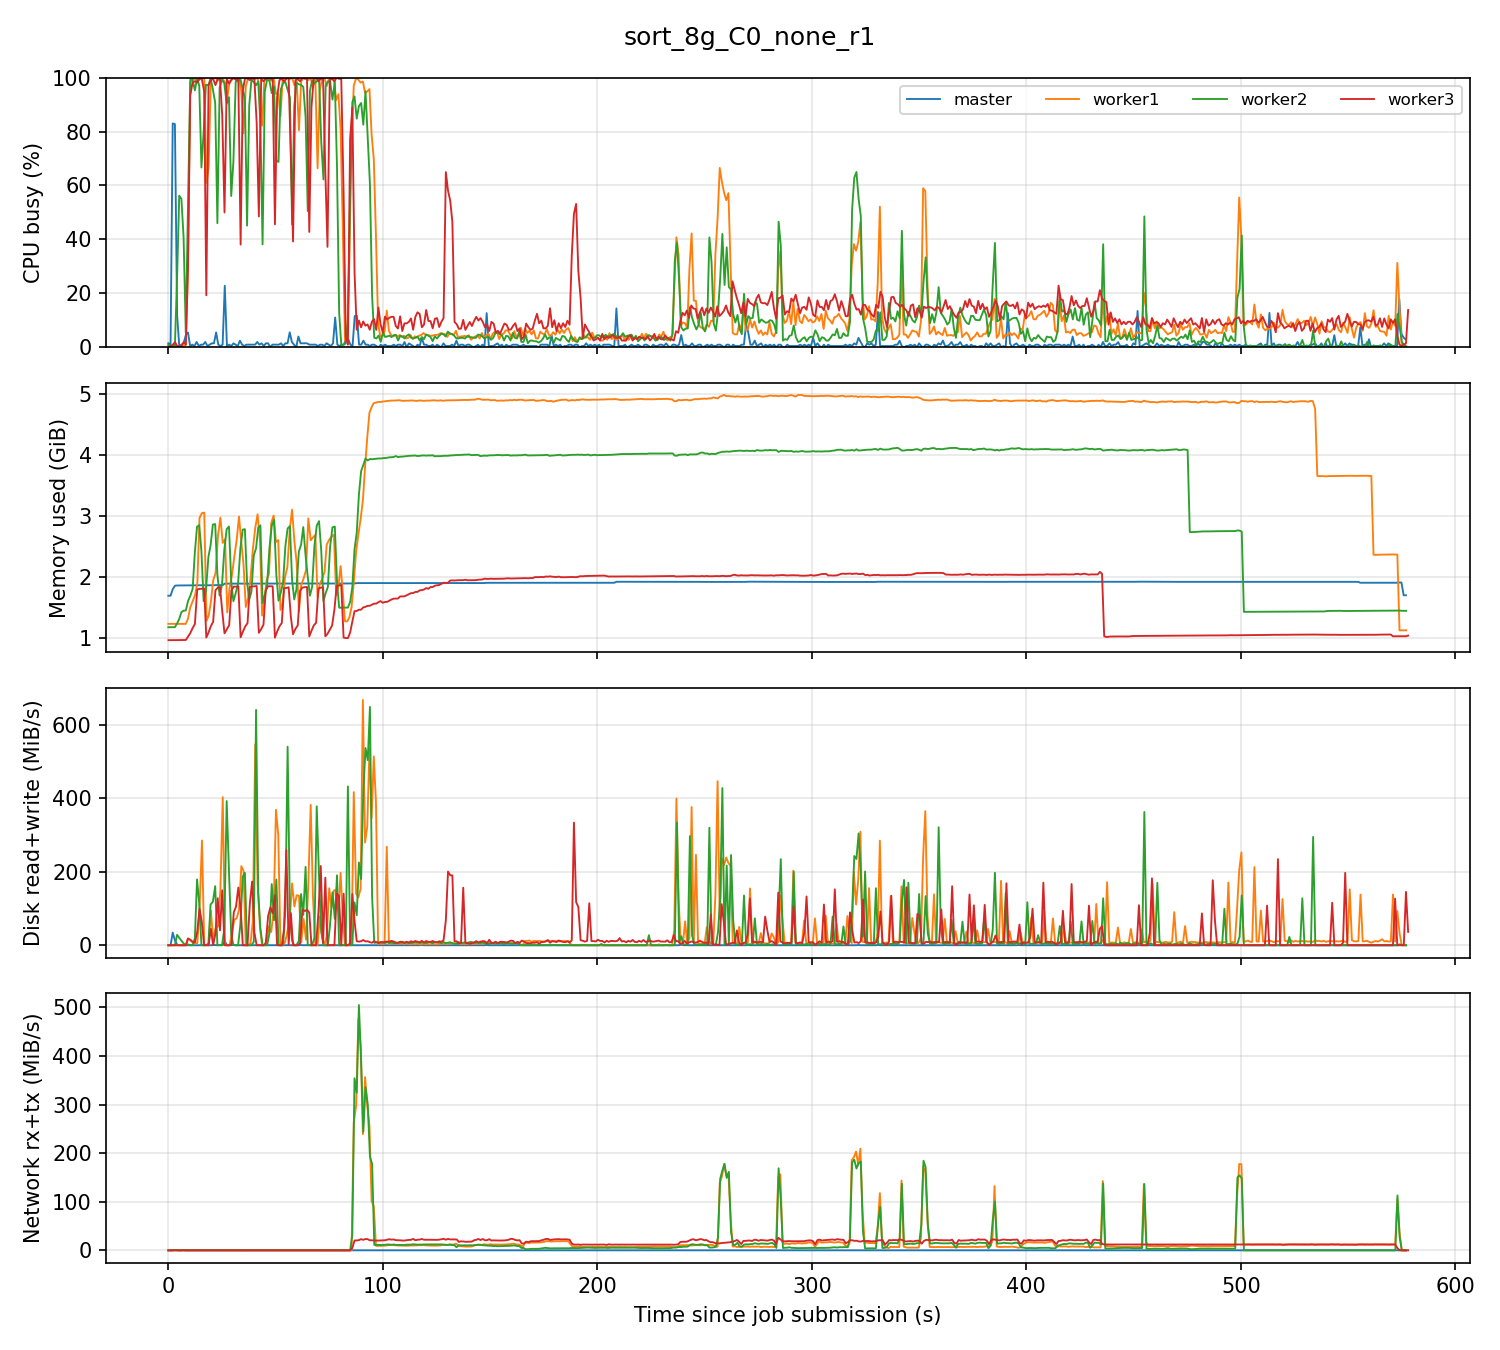
\includegraphics[width=0.85\linewidth]{../results/figures/monitor_sort_8g_C0_none_r1.png}
  \caption{Output of our monitor for one Sort run (8 GB, no compression): CPU, memory, disk and network for each node, one sample per second.}
  \label{fig:mon}
\end{figure}

\subsection{Reproducibility}
The cluster is deployed with an Ansible playbook (\path{ansible/site.yml}) that installs Java and Hadoop, writes the configuration from templates and starts the daemons. The experiments are run by shell scripts in \path{scripts/}, and the analysis by two Python scripts (\path{analysis/parse.py} turns the raw files into CSV tables, \path{analysis/plots.py} draws the figures). The data generator uses a fixed seed, so every run reads exactly the same records. The whole campaign is started with one command (\path{scripts/run_all.sh}) and a run that already has results is skipped, so the campaign can be resumed after an interruption. All raw measurements are in \path{results/raw/}, one directory per run.

\section{Methodology}
\subsection{Dataset}
The input is synthetic sales data. Each record is a line \path{id|date|city|product|price|qty|comment} where the id is a random 64-bit hex number and the comment is a sequence of words taken from a 20,000-word vocabulary with a Zipf distribution, so the text compresses roughly like real text. A map-only job (\path{DataGen}) writes the records into SequenceFiles with block compression. Each map task writes one file of about 100 MB, which is smaller than one HDFS block, so every codec gives the same number of input splits (11, 21, 41 and 82 for 1, 2, 4 and 8 GB). Block-compressed SequenceFiles are splittable for all codecs, including Gzip.

We used dataset sizes of 1, 2, 4 and 8 GB of raw text (the uncompressed SequenceFile of the 8 GB dataset is 8.4 GiB on HDFS). In the rest of the report, measured volumes are given in GiB. We did not go up to 20 GB because of time and disk space: the 468 runs of the campaign already took 37.6 hours, and the 18 datasets use 97 GiB of HDFS space with replication.

\subsection{Compression configurations}
Storage compression means that the input dataset is stored compressed with the codec and that the job also writes its output compressed with the same codec (\path{mapreduce.output.fileoutputformat.compress}, block type). Communication compression means that the map output is compressed before it is spilled to disk and sent to the reducers (\path{mapreduce.map.output.compress}). The four configurations are the ones of the project description:

\begin{table}[H]
  \centering
  \small
  \caption{Compression configurations}
  \begin{tabularx}{\linewidth}{lXl}
  \toprule
  \textbf{Config} & \textbf{Storage (HDFS input and output)} & \textbf{Communication (shuffle)} \\
  \midrule
  C0 & off & off \\
  C1 & on & off \\
  C2 & off & on \\
  C3 & on & on \\
  \bottomrule
  \end{tabularx}
\end{table}

For C1, C2 and C3 we tested the four codecs, so each application and size has 13 configurations (C0 plus 3 x 4). With 3 applications, 4 sizes and 3 repetitions this gives 468 runs.

\subsection{Running a measurement}
For every run the driver script drops the page cache on all nodes, starts the monitor on every node, submits the job, waits for it, stops the monitor and downloads the counters. The loop over repetitions is the outer loop: we first run every configuration once, then every configuration a second time, and so on. This way a slow period of the hosts (for example a background update on the PC) affects one repetition of many configurations instead of all repetitions of one configuration. Graphs show the mean of the 3 runs and error bars show the standard deviation. Across all configurations, the median coefficient of variation of the execution time is 6.7\%.

\subsection{Metrics}
\begin{itemize}
  \item Execution time: finish time minus start time of the job, from JobHistory.
  \item CPU consumption: the \path{CPU_MILLISECONDS} counter, which is the CPU time of all map and reduce tasks.
  \item CPU utilization: the share of the workers' CPU time that was busy during the job, from the monitor.
  \item Disk I/O volume: bytes read plus bytes written on the disks of the three workers, from the monitor.
  \item Network traffic: bytes sent by all nodes, from the monitor.
  \item Shuffle volume and time: \path{REDUCE_SHUFFLE_BYTES} and the average shuffle time of the reduce tasks.
  \item Compressed dataset size: size of the dataset directory on HDFS.
\end{itemize}

\section{Workloads and their characterization}
The three applications are written in Java with the MapReduce API. They all read the same SequenceFiles and use 6 reducers.

\begin{itemize}
  \item Sort (I/O-bound): a total-order sort of all records. The map emits the record as the key, a range partitioner on the first byte of the id sends each range to one reducer, and the reducer writes the records back. There is almost no computation, but the whole dataset is read, shuffled and written again (with 2 replicas).
  \item HashScore (CPU-bound): for each record the map computes 1,000 rounds of SHA-256 and emits the city and a small score. A combiner sums the scores, so only 20 keys per map task are shuffled and the output is tiny.
  \item BigramCount (balanced): the map splits the comment into words and emits every pair of consecutive words with a count of 1. A combiner and the reducer sum the counts. The application does real work on every record and also shuffles several GB.
\end{itemize}

Table 3 shows the measurements that support this classification, for the 8 GB dataset without compression. Sort uses only 19\% of the worker CPUs but moves 94 MB/s on disk and 25 MB/s on the network. HashScore keeps the CPUs 80\% busy and hardly uses the network (0.01 MB/s). BigramCount is in between, with 54\% CPU and almost as much disk traffic as Sort. Figure~\ref{fig:char} shows the same thing over time: the CPU of HashScore stays above 90\% for the whole map phase, while Sort has a short CPU peak during the map phase and then a long reduce phase where the CPUs are almost idle and the job waits for data.

\begin{table}[H]
  \centering
  \small
  \caption{Characterization of the applications (8 GB, C0, mean of 3 runs)}
  \begin{tabular}{lrrrrr}
  \toprule
  \textbf{Application} & \textbf{Exec. time (s)} & \textbf{CPU time (s)} & \textbf{CPU util.} & \textbf{Disk (MB/s)} & \textbf{Network (MB/s)} \\
  \midrule
  Sort & 585 & 517 & 19\% & 93.6 & 24.6 \\
  HashScore & 745 & 5,795 & 80\% & 12.1 & 0.01 \\
  BigramCount & 468 & 2,086 & 54\% & 79.5 & 14.3 \\
  \bottomrule
  \end{tabular}
\end{table}

\begin{figure}[H]
  \centering
  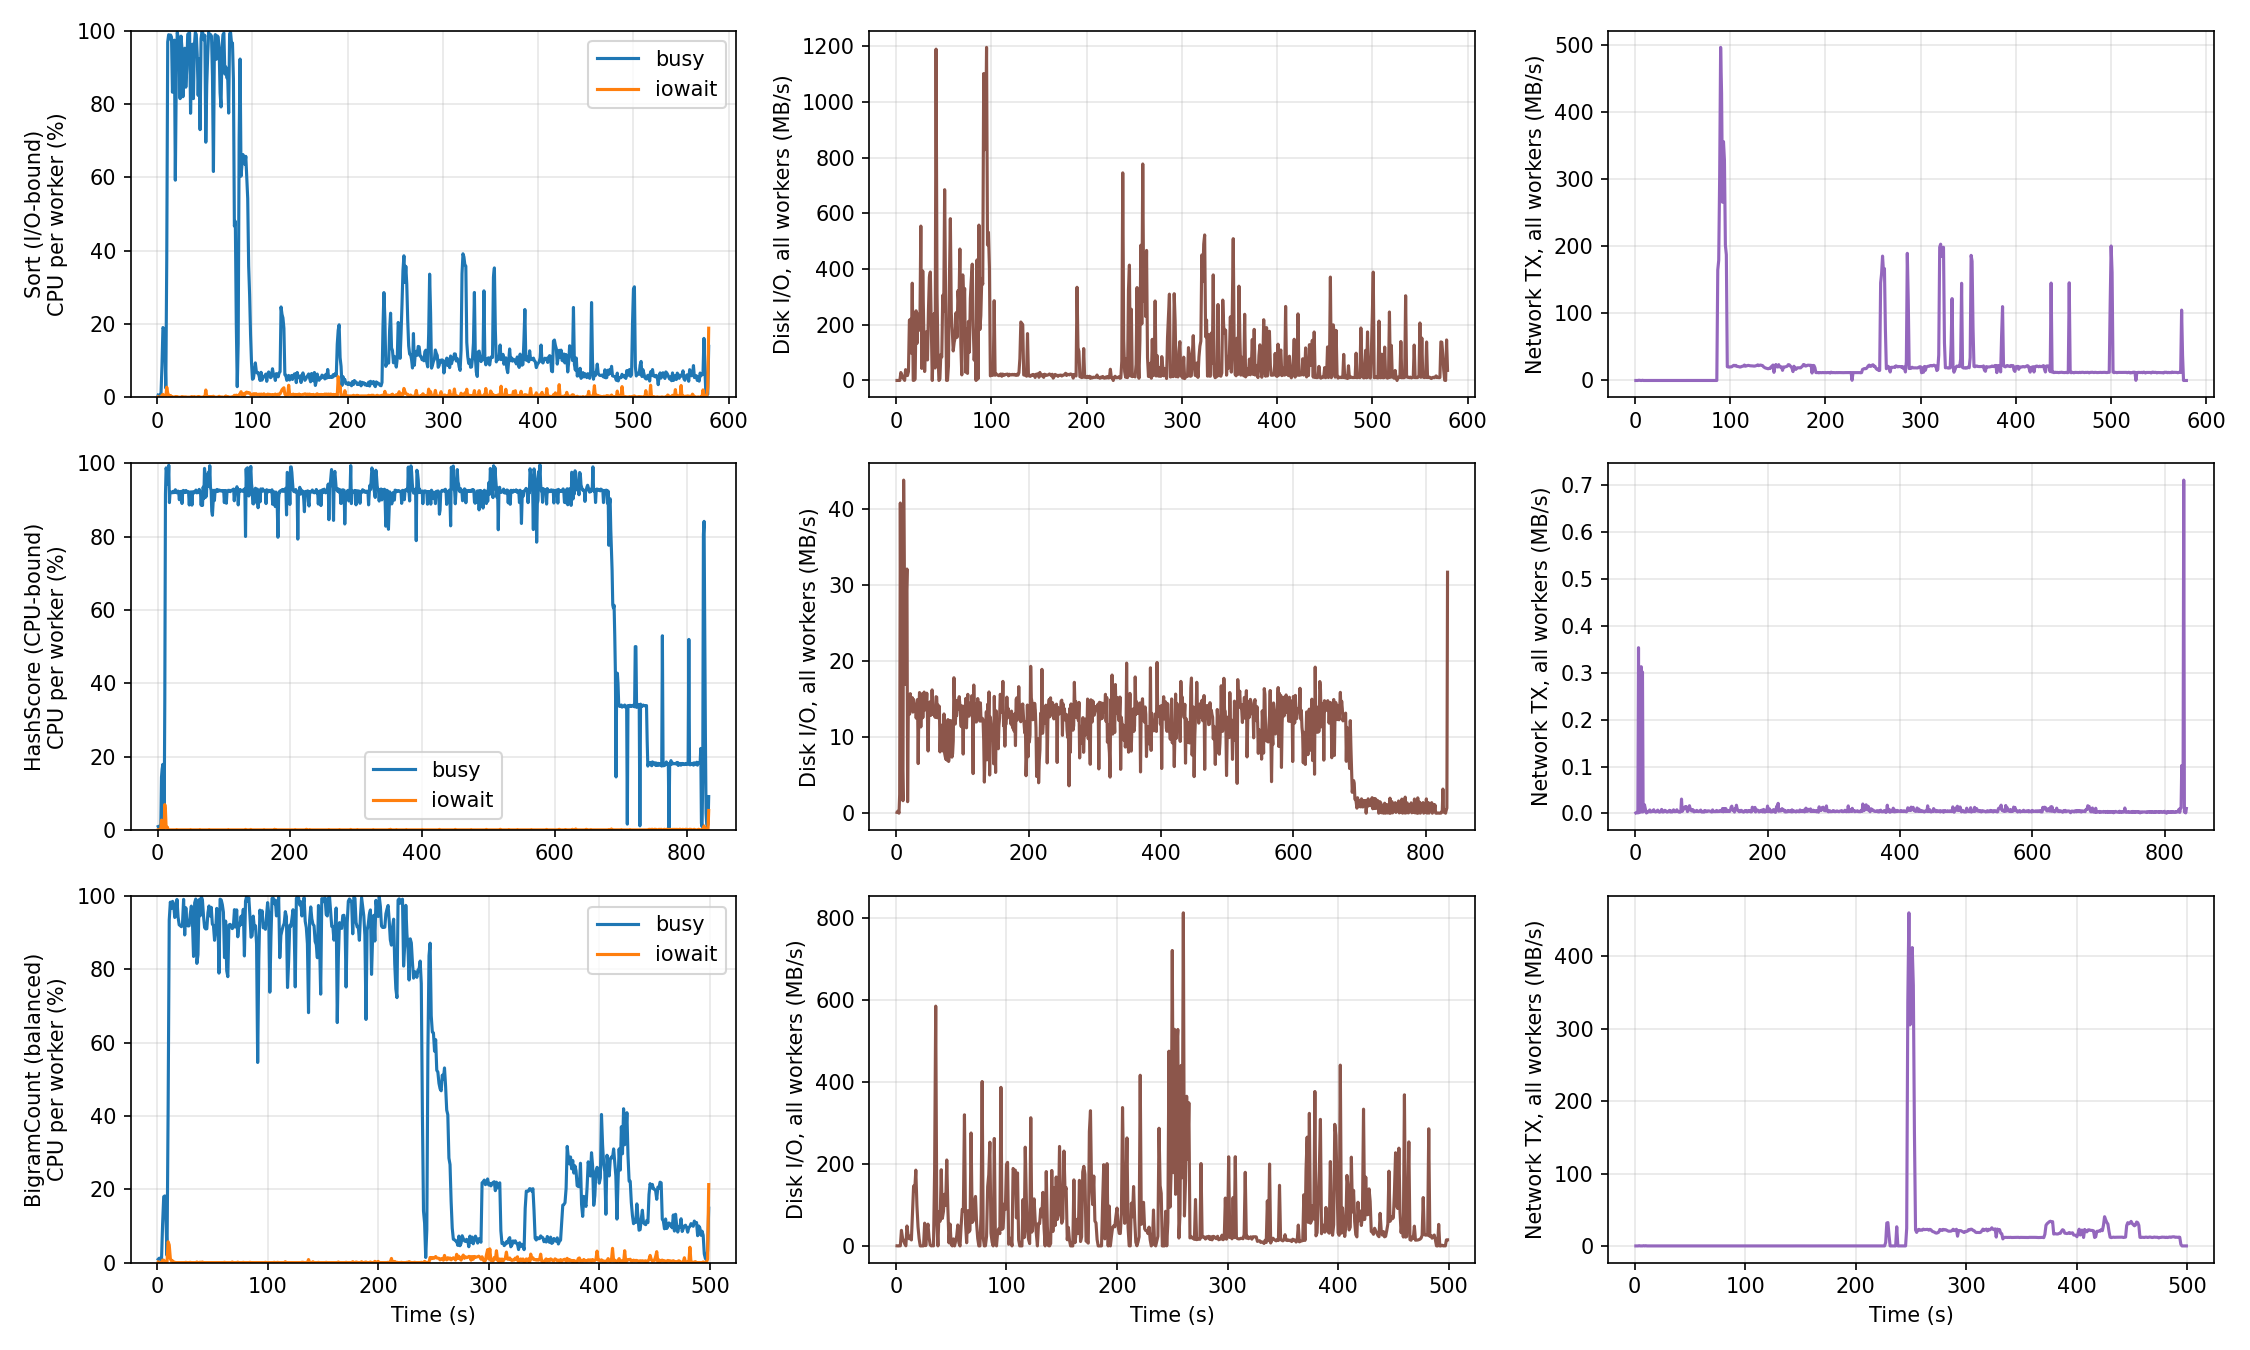
\includegraphics[width=1\linewidth]{../results/figures/characterization_timeseries.png}
  \caption{CPU, disk and network over time for the three applications (8 GB, C0). CPU is the average of the workers, disk and network are summed over the workers.}
  \label{fig:char}
\end{figure}

The iowait values are very low for all applications (below 0.5\%). The virtual disks of the PC workers are files on an NVMe SSD and the page cache of the host absorbs part of the writes, so the disks themselves are rarely the limit. For Sort, the real limit is the network link of worker3. In Figure~\ref{fig:mon} the reduce phase of Sort lasts from about 100 s to 580 s; during this time no node is CPU-bound and worker3 sends and receives a constant 12 MB/s, which is the speed of a 100 Mbit/s link. The other reducers wait for the map output stored on worker3 and the output blocks replicated to it. We come back to this in the discussion, because it explains why compression helps Sort so much on our cluster.

\section{Intrinsic characteristics of the codecs}
Before using the codecs in jobs, we measured them alone with a small Java program (\path{CodecBench}) that calls the same Hadoop codec classes. It compresses and decompresses a 256 MB sample of our dataset on one thread, 5 times, and measures the wall time and the CPU time of the thread. We also tested Zstandard at levels 1, 9 and 19 to see the range of this codec. Table 4 gives the results.

\begin{table}[H]
  \centering
  \small
  \caption{Codec micro-benchmark (256 MB sample, one core, mean of 5 runs)}
  \begin{tabularx}{\linewidth}{lrrrX}
  \toprule
  \textbf{Codec} & \textbf{Ratio} & \textbf{Compr. (MB/s)} & \textbf{Decompr. (MB/s)} & \textbf{CPU s per GB (compr. + decompr.)} \\
  \midrule
  Snappy & 1.56 & 438 & 1,280 & 3.2 \\
  LZ4 & 1.51 & 474 & 2,982 & 2.6 \\
  Gzip & 2.35 & 34 & 201 & 35.1 \\
  Zstd level 1 & 2.28 & 289 & 1,228 & 4.4 \\
  Zstd level 3 (used) & 2.59 & 181 & 1,208 & 6.6 \\
  Zstd level 9 & 2.82 & 31 & 1,005 & 34.3 \\
  Zstd level 19 & 3.20 & 2.0 & 828 & 501 \\
  \bottomrule
  \end{tabularx}
\end{table}

Snappy and LZ4 are the fastest codecs, about 450 MB/s for compression, but they only reduce the data by about a third (ratio around 1.55). LZ4 decompresses more than twice as fast as Snappy. Gzip reaches a ratio of 2.35 but compresses at only 34 MB/s, so it costs 11 times more CPU per GB than Snappy. Zstandard at level 3 compresses better than Gzip (2.59) while being 5 times faster to compress and 6 times faster to decompress. Higher Zstandard levels give a better ratio but compression becomes very slow (2 MB/s at level 19), so they are only useful for data that is written once and read many times.

The ratios measured on HDFS with the real datasets are very close: 1.60 for Snappy, 1.55 for LZ4, 2.37 for Gzip and 2.55 for Zstandard (Figure~\ref{fig:ratio}). The 8 GB dataset takes 8.41 GiB uncompressed, 5.26 GiB with Snappy, 5.42 GiB with LZ4, 3.55 GiB with Gzip and 3.30 GiB with Zstandard. Interestingly, writing the dataset was faster with every codec than without compression, even with Gzip (150 s instead of 352 s for 8 GB), because writing 9 GB twice to HDFS costs more than the CPU time of compression.

\begin{figure}[H]
  \centering
  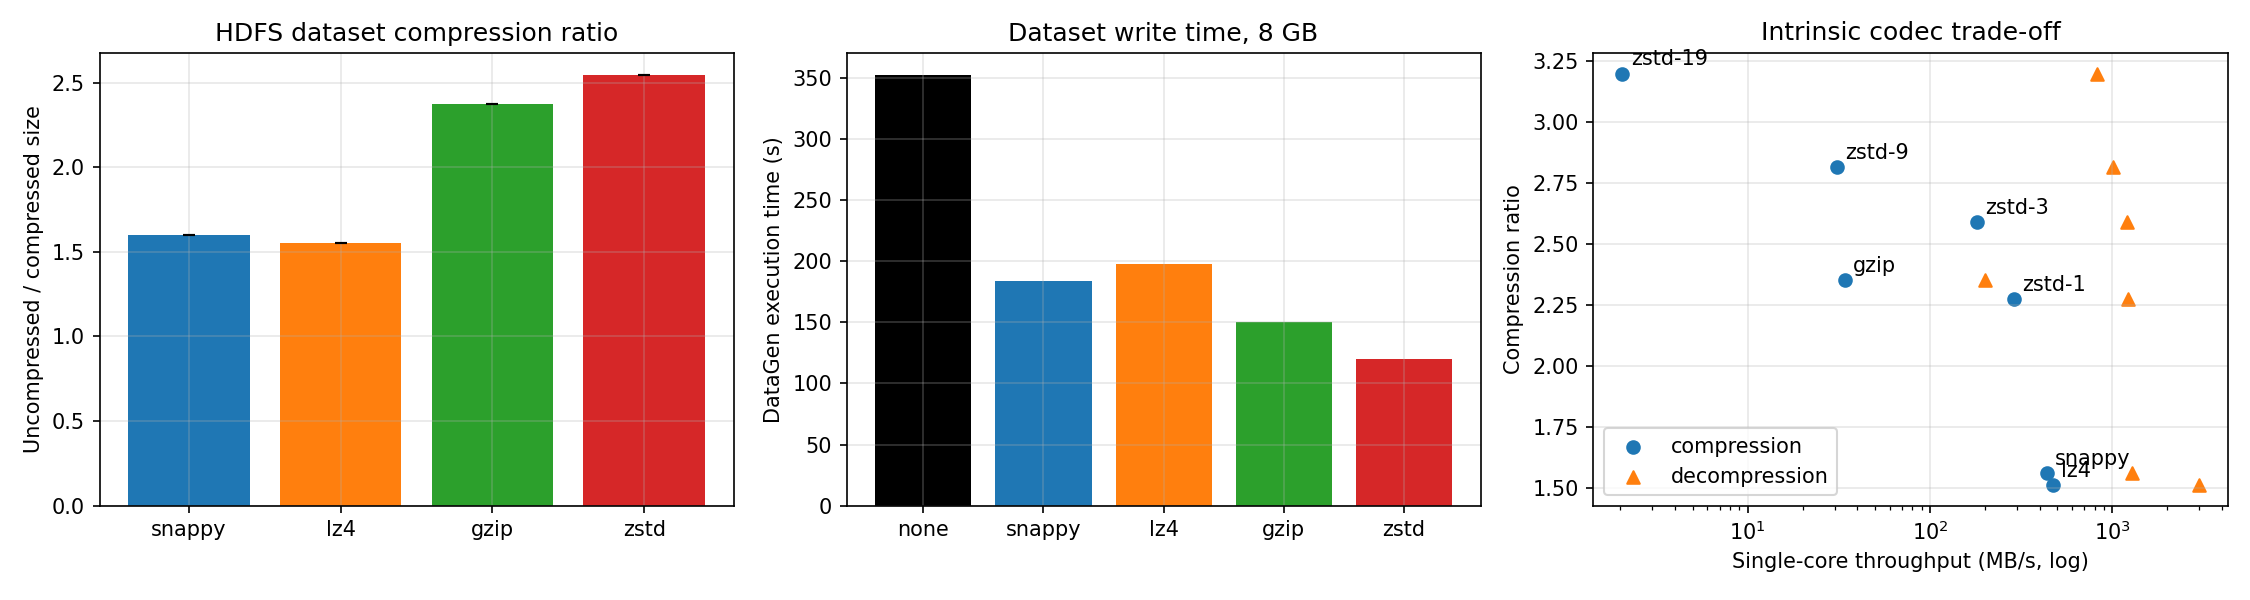
\includegraphics[width=1\linewidth]{../results/figures/compression_ratio.png}
  \caption{Left: compression ratio of the datasets on HDFS. Middle: time to generate and write the 8 GB dataset. Right: ratio against single-core throughput from the micro-benchmark.}
  \label{fig:ratio}
\end{figure}

\section{Storage-level compression (C1)}
The following figures show execution time, CPU time, disk volume and network traffic against the dataset size. In each figure the left panel is storage compression (C1) and the right panel is shuffle compression (C2), both compared with C0.

\begin{figure}[H]
  \centering
  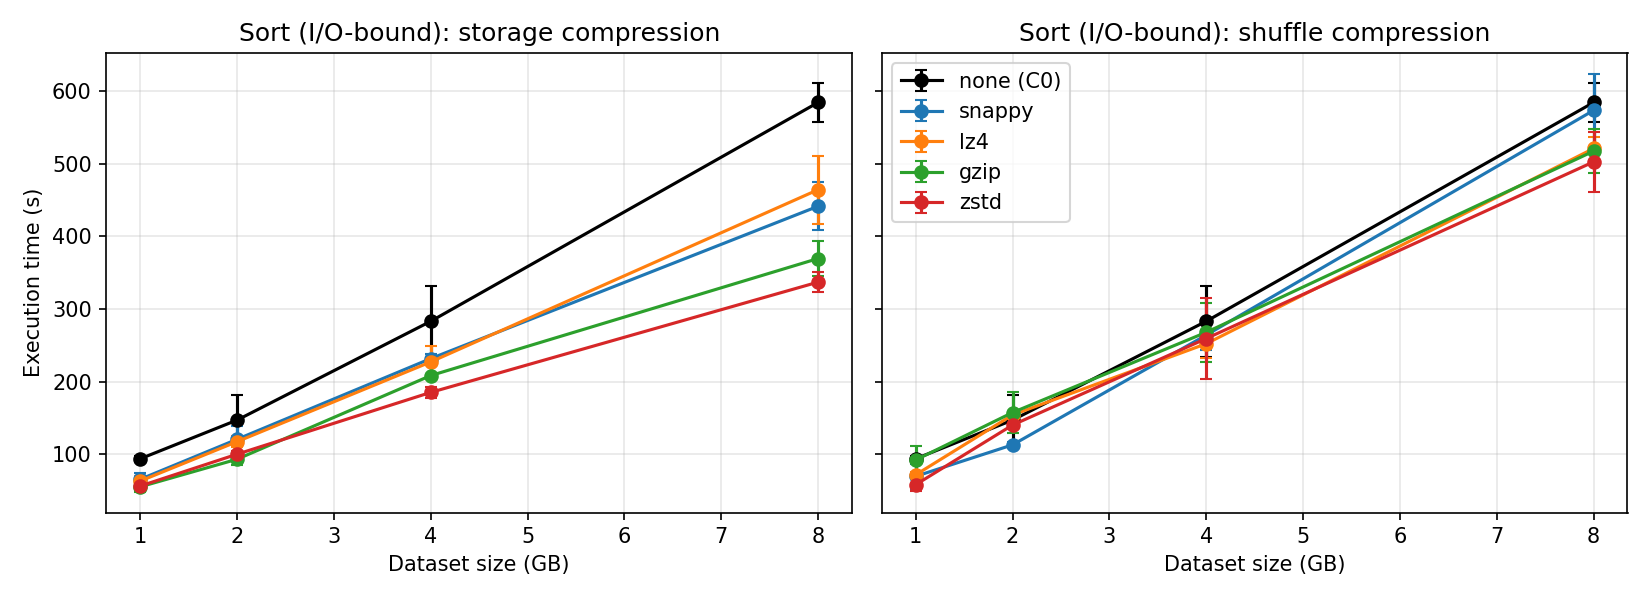
\includegraphics[width=0.9\linewidth]{../results/figures/exec_vs_size_sort.png}
  \caption{Sort: execution time against dataset size.}

\end{figure}

\begin{figure}[H]
  \centering
  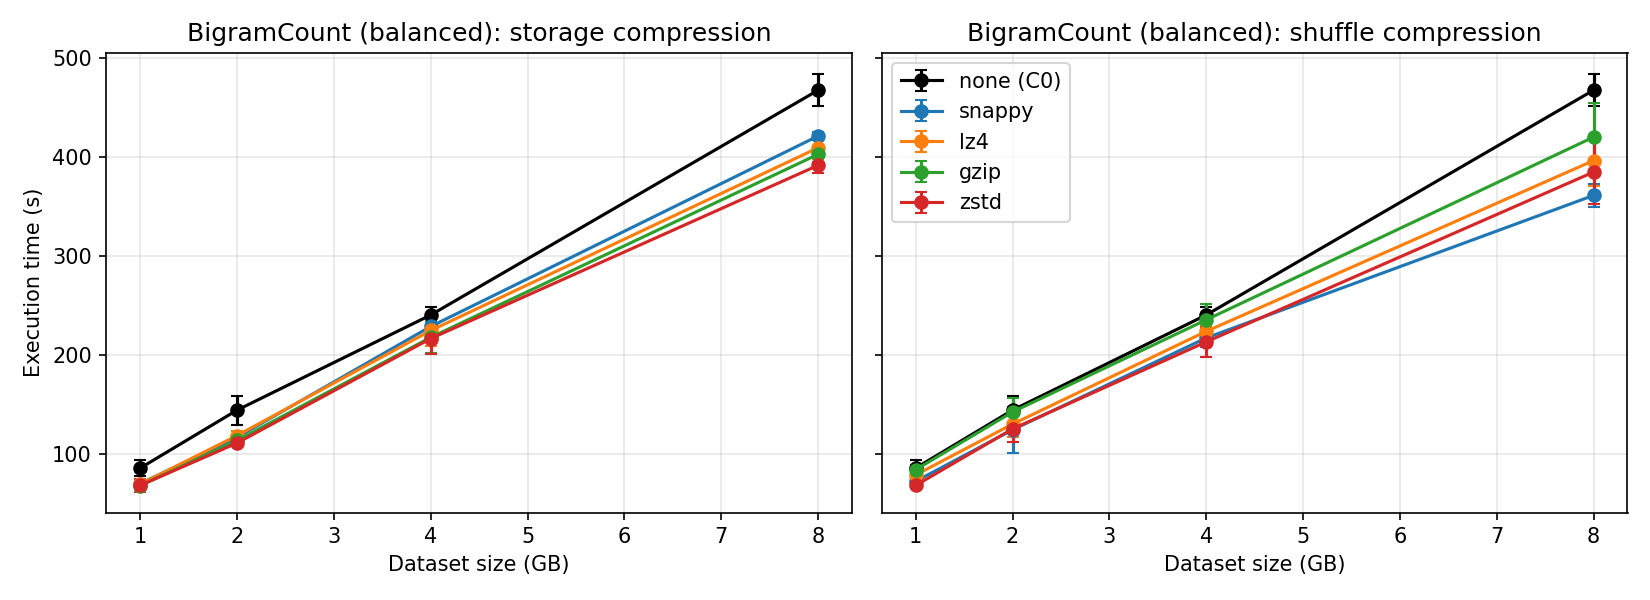
\includegraphics[width=0.9\linewidth]{../results/figures/exec_vs_size_bigram.png}
  \caption{BigramCount: execution time against dataset size.}

\end{figure}

\begin{figure}[H]
  \centering
  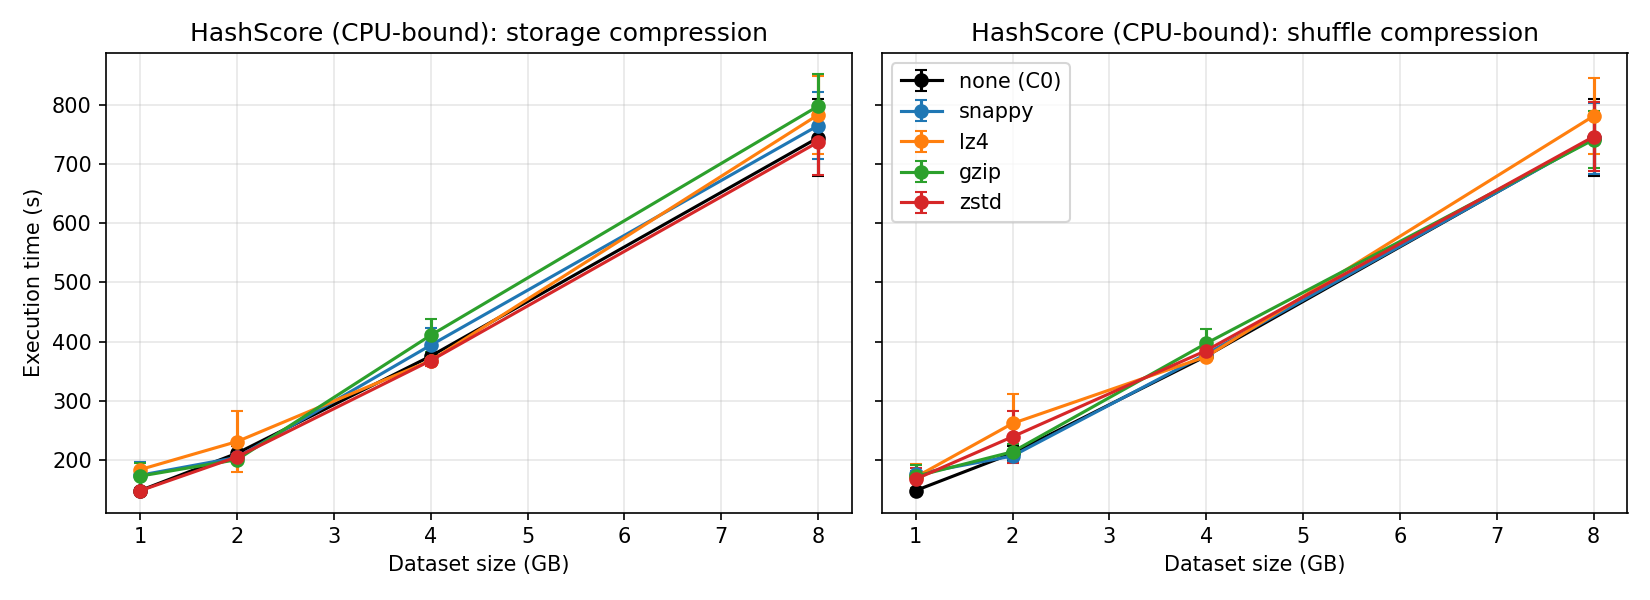
\includegraphics[width=0.9\linewidth]{../results/figures/exec_vs_size_hashscore.png}
  \caption{HashScore: execution time against dataset size.}

\end{figure}

Storage compression makes Sort much faster. With 8 GB, the execution time goes from 585 s (C0) to 442 s with Snappy, 464 s with LZ4, 370 s with Gzip and 337 s with Zstandard, which is 20\% to 42\% less. Two things reduce the I/O. First, the input that the maps read from HDFS is smaller (3.3 GiB instead of 8.4 GiB with Zstandard). Second, Sort writes an output as large as its input, and with C1 this output is also compressed, so both replicas are smaller and less data has to cross the network. The disk volume of the workers drops from 54 GiB to 33 GiB with Zstandard and the network traffic from 14.2 GiB to 8.8 GiB (Figure~\ref{fig:disksort} and Figure~\ref{fig:netsort}). The average reduce time drops from 300 s to 74 s.

BigramCount gains less: 10\% (Snappy) to 16\% (Zstandard) at 8 GB. Its output is small, so C1 only reduces the input read. HashScore does not gain anything: the results are between 1\% faster (Zstandard) and 7\% slower (Gzip), which is inside the run-to-run variation of this application (standard deviation around 55 to 65 s, or 8\%).

\begin{figure}[H]
  \centering
  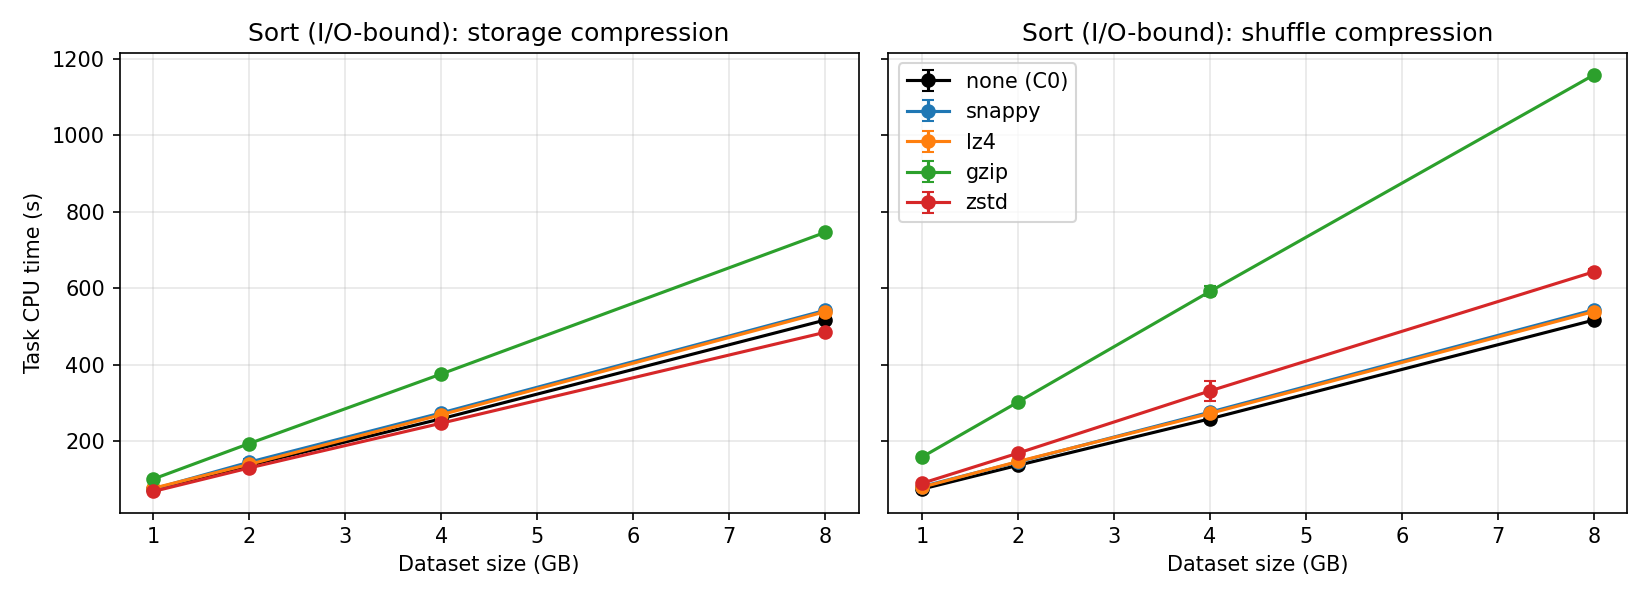
\includegraphics[width=0.9\linewidth]{../results/figures/cpu_vs_size_sort.png}
  \caption{Sort: total task CPU time against dataset size.}

\end{figure}

\begin{figure}[H]
  \centering
  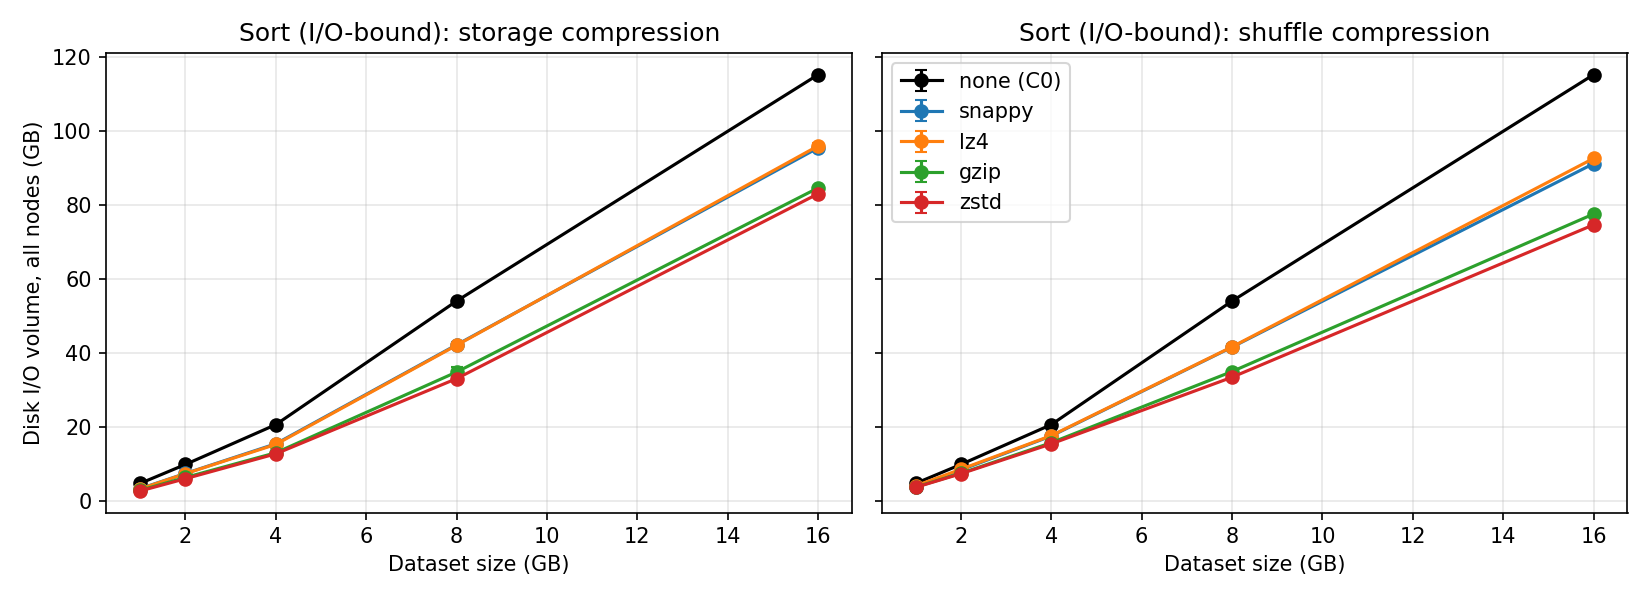
\includegraphics[width=0.9\linewidth]{../results/figures/disk_vs_size_sort.png}
  \caption{Sort: disk volume (read + written, all workers) against dataset size.}
  \label{fig:disksort}
\end{figure}

Does the reduction of disk I/O compensate for the extra CPU cost? For Snappy, LZ4 and Zstandard the extra CPU is very small: the CPU time of Sort at 8 GB is 517 s without compression, 542 s with Snappy, 538 s with LZ4, and even a bit lower with Zstandard (485 s), because the tasks also have fewer bytes to read, copy and checksum. Gzip is the exception: it adds 44\% of CPU time (746 s). Even so, Gzip is the second fastest codec for Sort in C1, because the cluster has idle CPU during the I/O-bound phases. So on our cluster the answer is yes for every codec on Sort and BigramCount, and the gain is larger for the codecs with a better ratio. For HashScore there is no I/O to save, so the CPU cost is not compensated, but it is also small compared with the 5,800 s of CPU time of the application.

\section{Communication-level compression (C2)}
\begin{figure}[H]
  \centering
  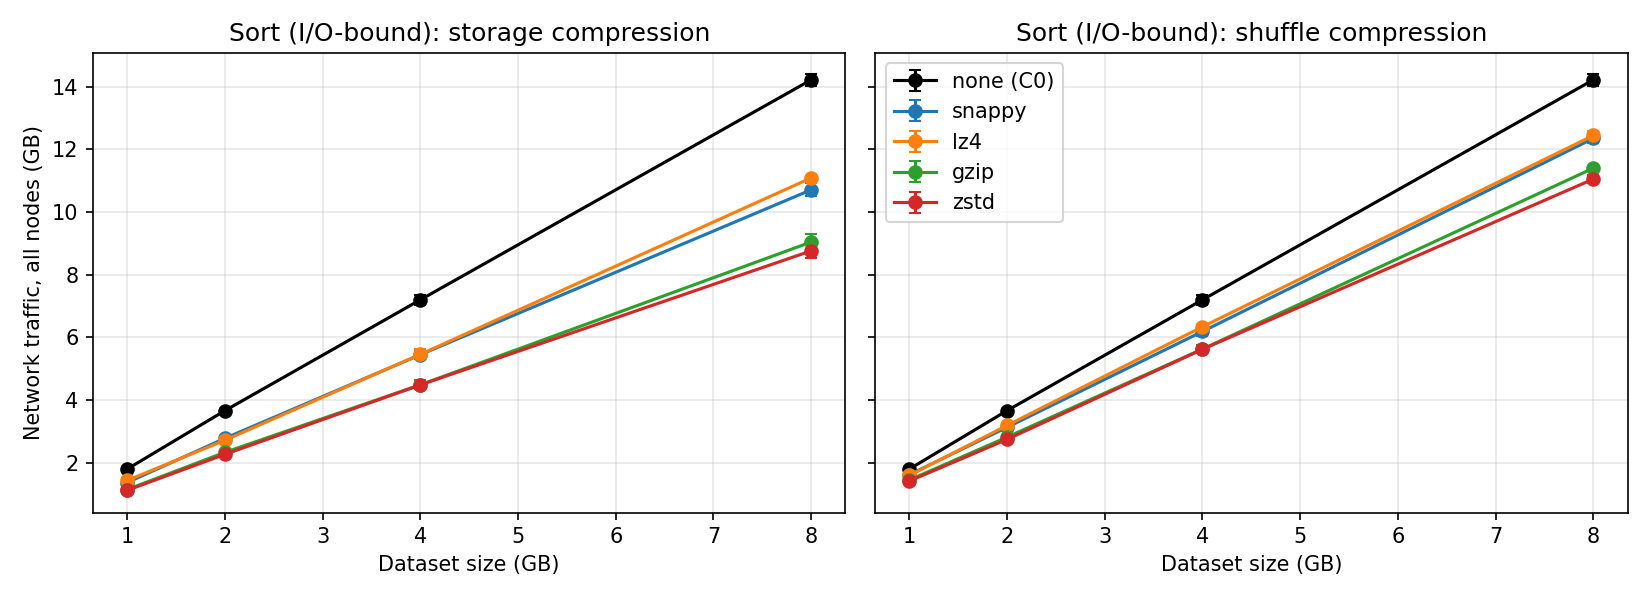
\includegraphics[width=0.9\linewidth]{../results/figures/net_vs_size_sort.png}
  \caption{Sort: network traffic (bytes sent by all nodes) against dataset size.}
  \label{fig:netsort}
\end{figure}

\begin{figure}[H]
  \centering
  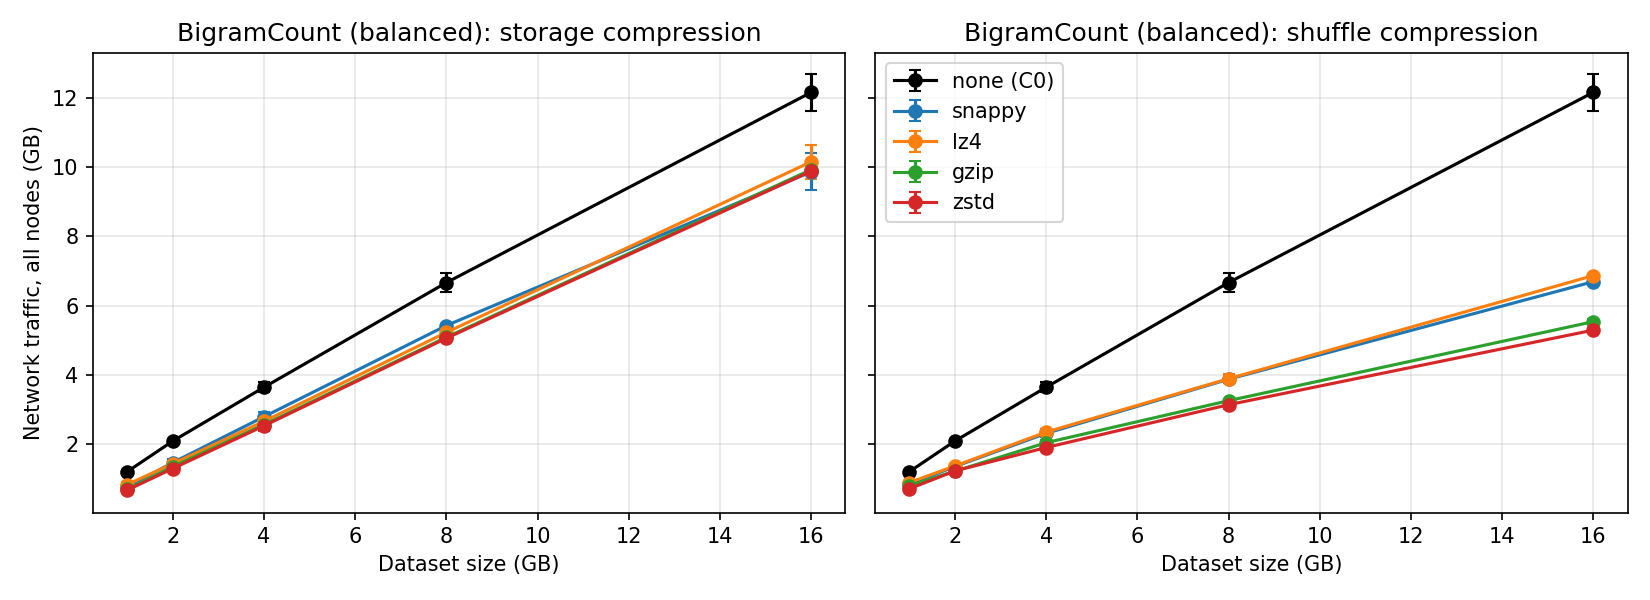
\includegraphics[width=0.9\linewidth]{../results/figures/net_vs_size_bigram.png}
  \caption{BigramCount: network traffic against dataset size.}

\end{figure}

Shuffle compression reduces the volume of the shuffle in the same proportion as the ratios of Table 4. For Sort at 8 GB, the 8.2 GiB of map output becomes 5.2 GiB with Snappy, 5.4 GiB with LZ4, 3.5 GiB with Gzip and 3.1 GiB with Zstandard, and the average shuffle time of the reducers goes from 138 s to 60 s with Zstandard (Figure~\ref{fig:shtime}). For BigramCount the shuffle goes from 6.9 GiB to between 1.5 GiB (Zstandard) and 2.7 GiB (LZ4), and the total network traffic is cut by half. HashScore shuffles only a few kilobytes, so C2 changes nothing for it.

\begin{figure}[H]
  \centering
  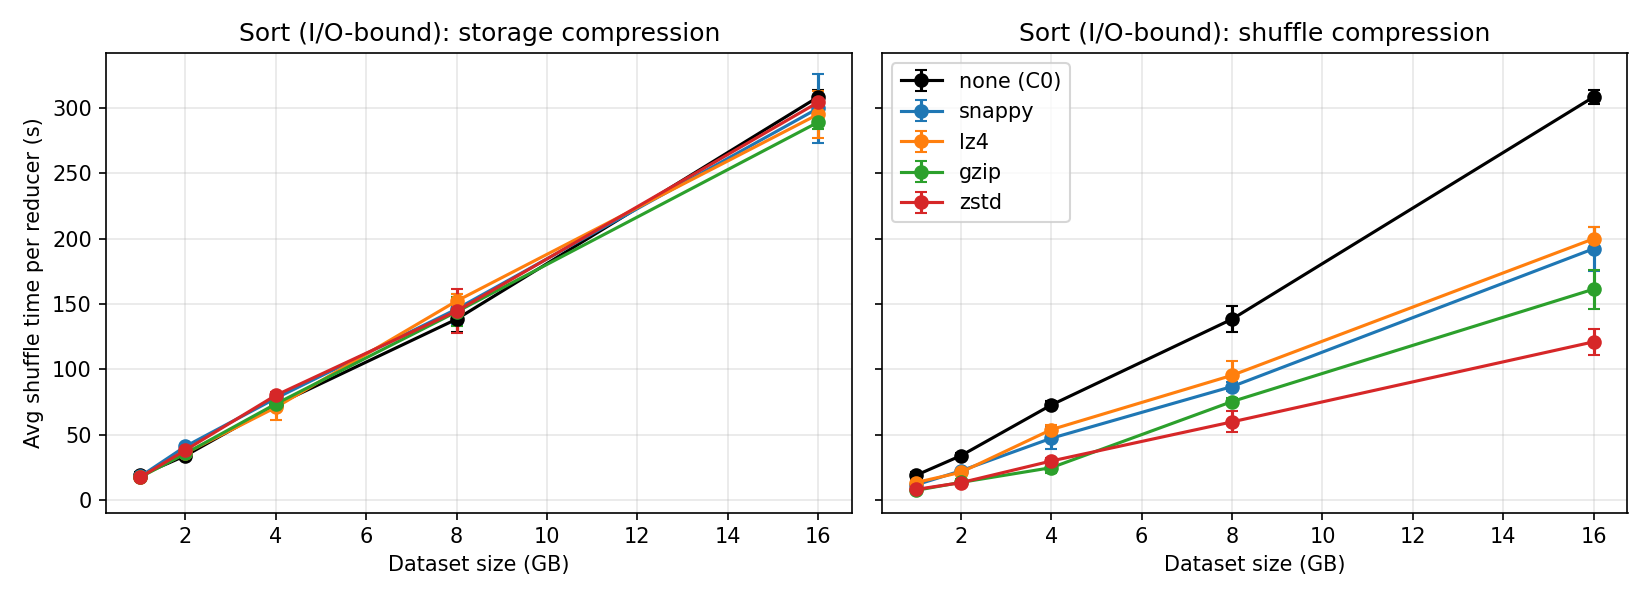
\includegraphics[width=0.9\linewidth]{../results/figures/shuffle_time_vs_size_sort.png}
  \caption{Sort: average shuffle time of the reduce tasks against dataset size.}
  \label{fig:shtime}
\end{figure}

\begin{figure}[H]
  \centering
  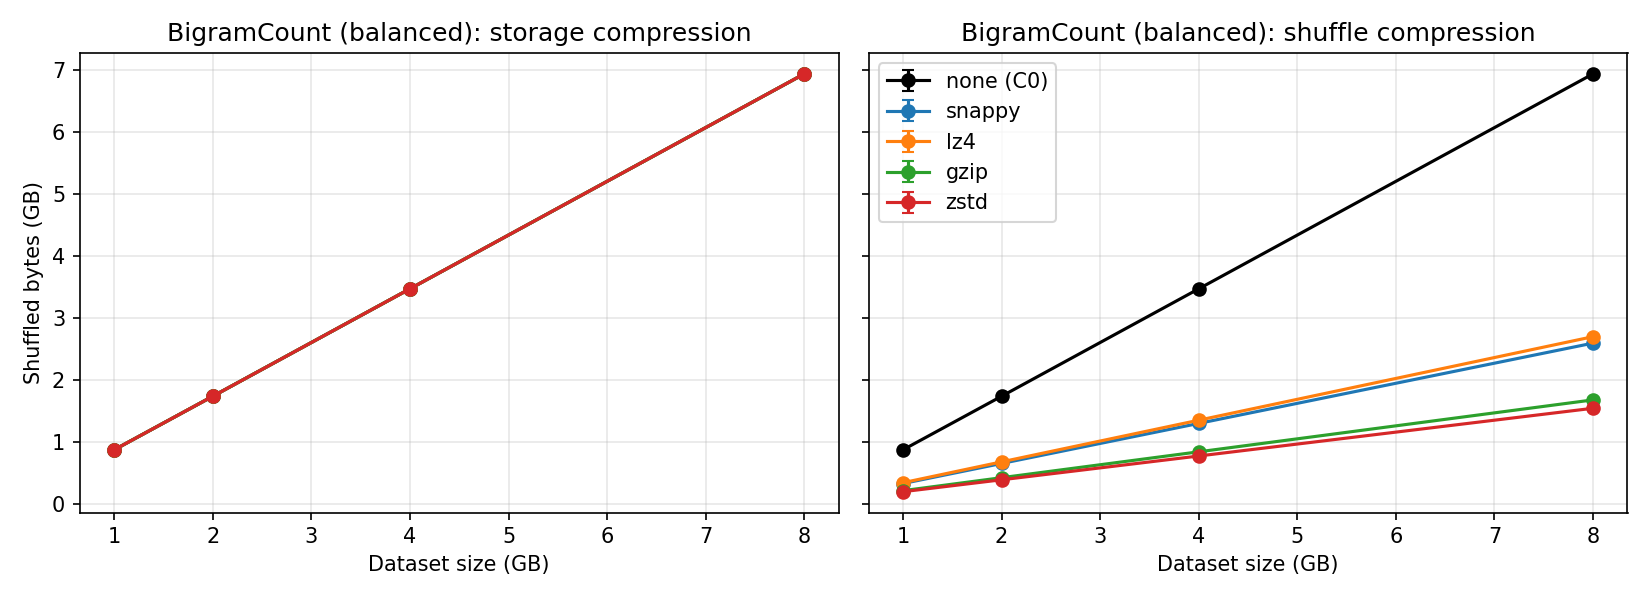
\includegraphics[width=0.9\linewidth]{../results/figures/shuffle_bytes_vs_size_bigram.png}
  \caption{BigramCount: shuffled bytes against dataset size.}

\end{figure}

The effect on the total execution time is smaller than on the shuffle. For BigramCount, C2 saves 10\% (Gzip) to 23\% (Snappy) at 8 GB. For Sort it saves 2\% (Snappy) to 14\% (Zstandard), and the error bars are large. There are two reasons. First, the shuffle is only one part of the data movement of Sort: the input read and the replicated output are not affected by C2. Second, compressing the map output costs CPU in the map tasks and decompressing it costs CPU in the reducers. With Gzip, the CPU time of Sort more than doubles (1,158 s instead of 517 s) and the map phase becomes slower (average map time 10.5 s instead of 7.1 s). With Zstandard the CPU time goes up by 24\% and with Snappy and LZ4 by only 4\% to 5\%.

Compression of the shuffle becomes counterproductive when its CPU cost is larger than the time saved on the transfer. This almost happens with Gzip on Sort, where the large CPU overhead eats most of the gain, and it would happen on a cluster with a fast network and busy CPUs. In the main campaign the PC workers exchange data through a virtual switch that is much faster than a real network, which hides part of the benefit of C2. To check this, we repeated the C2 experiments with the network limited to 100 Mbit/s (next subsection).

\section{Combined compression (C3)}
\begin{figure}[H]
  \centering
  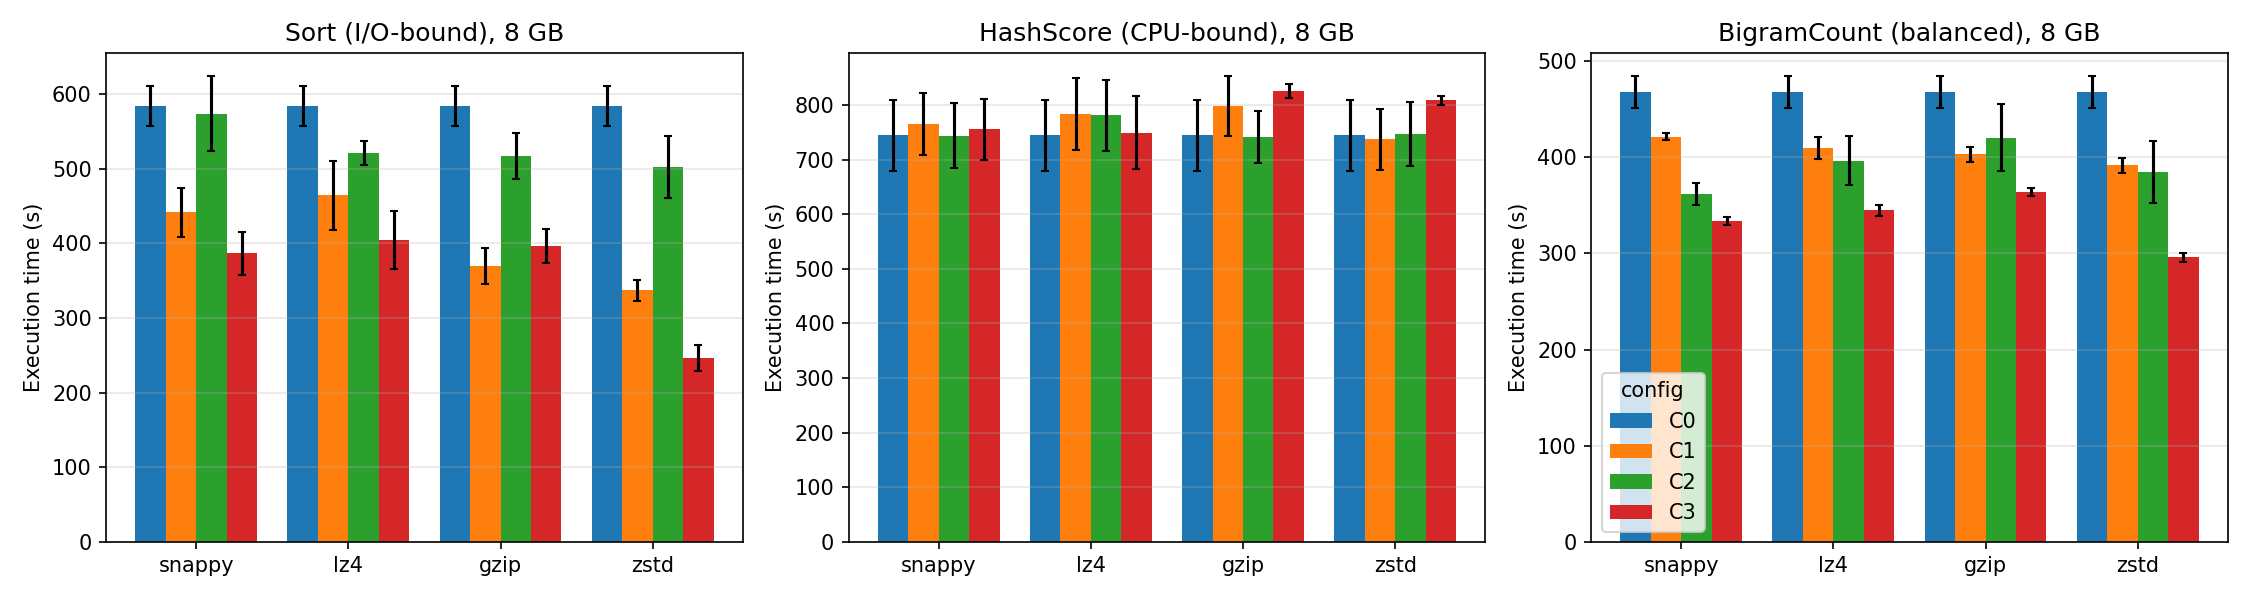
\includegraphics[width=1\linewidth]{../results/figures/exec_vs_config.png}
  \caption{Execution time for C0, C1, C2 and C3 with each codec, 8 GB.}
  \label{fig:config}
\end{figure}

Figure~\ref{fig:config} compares the four configurations at 8 GB. For Sort and BigramCount, C3 is the fastest configuration for every codec, with one exception (Gzip on Sort, see below). The best result overall is Sort with Zstandard in C3: 247 s instead of 585 s, which is 58\% less than C0 and 27\% less than C1 with the same codec. BigramCount with Zstandard in C3 takes 296 s instead of 468 s (37\% less). The gains of the two levels add up because they act on different bytes: C1 reduces the HDFS input and output, C2 reduces the shuffle.

Combining both levels can still make things worse. The clearest case is Gzip on Sort: C3 with Gzip takes 396 s while C1 with Gzip takes 370 s, so adding Gzip compression of the shuffle on top of Gzip storage compression costs 7\%. The same happens at 2 GB. The CPU time of Sort in C3 with Gzip is 1,395 s, 2.7 times the CPU time of C0. For HashScore, C3 is never better than C0 and it is the worst configuration with Gzip (+11\%) and Zstandard (+9\%). In these cases the job pays the CPU cost of compressing twice and gets nothing back, because the bottleneck is elsewhere.

\begin{figure}[H]
  \centering
  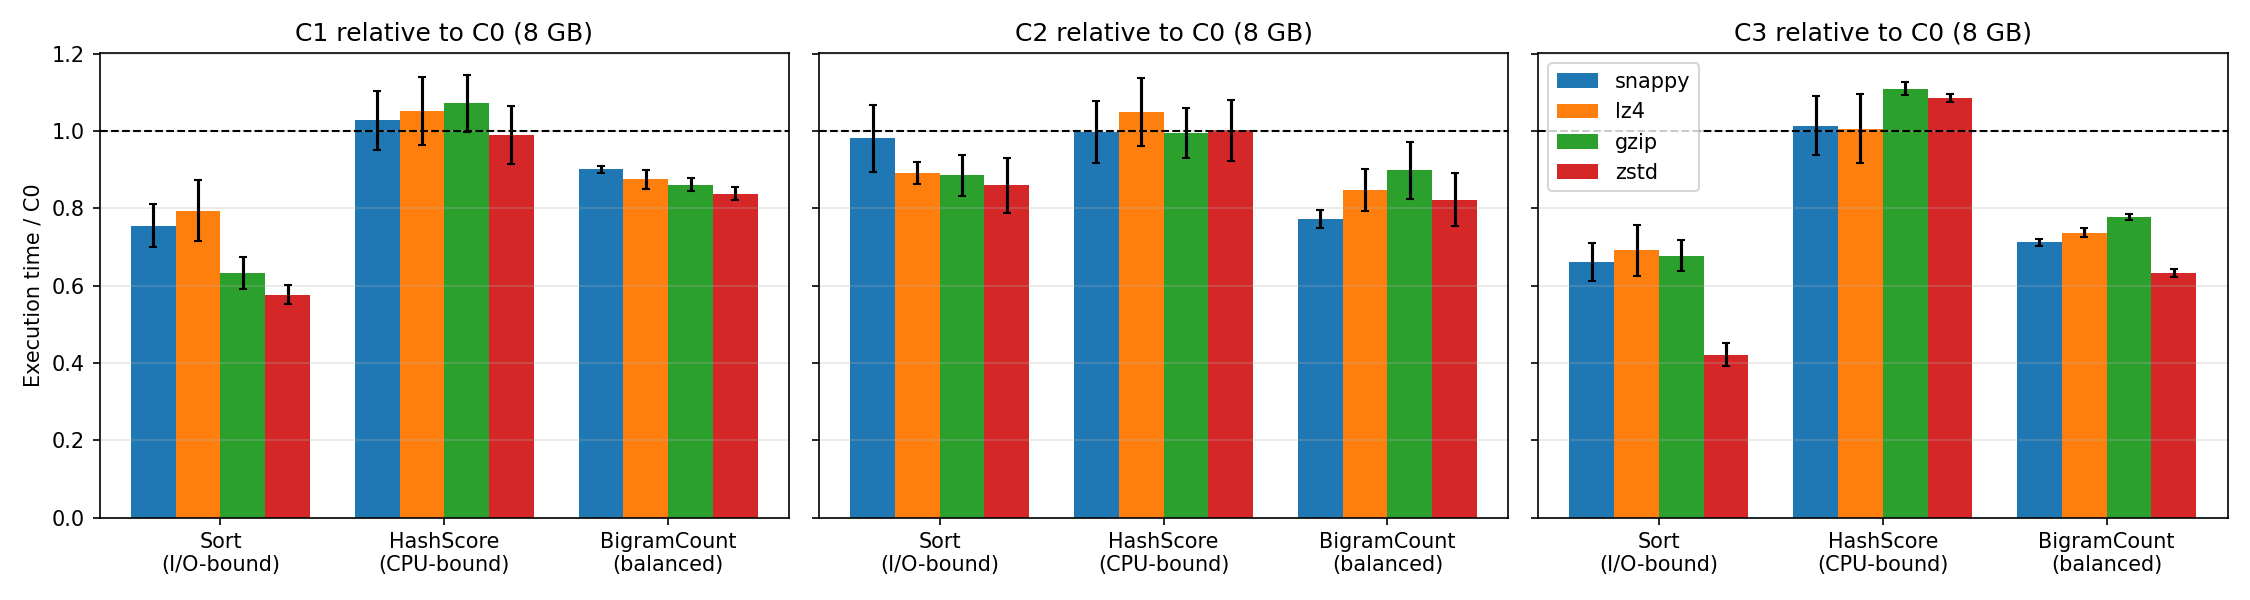
\includegraphics[width=1\linewidth]{../results/figures/exec_vs_workload.png}
  \caption{Execution time of C1, C2 and C3 divided by the execution time of C0, for each workload type (8 GB). Values below 1 mean that compression helps.}

\end{figure}

\section{Impact of dataset size}
Table 5 gives the change of execution time compared with C0 for every size, for the best codec of each application (Zstandard) and for the worst cases of HashScore. A negative value means that the job is faster.

\begin{table}[H]
  \centering
  \small
  \caption{Change of execution time compared with C0 (\%), mean of 3 runs}
  \begin{tabular}{lrrrr}
  \toprule
  \textbf{Application, config, codec} & \textbf{1 GB} & \textbf{2 GB} & \textbf{4 GB} & \textbf{8 GB} \\
  \midrule
  Sort, C1, Zstd & -40 & -32 & -35 & -42 \\
  Sort, C2, Zstd & -38 & -5 & -8 & -14 \\
  Sort, C3, Zstd & -56 & -53 & -49 & -58 \\
  Sort, C3, Gzip & -43 & -23 & -33 & -32 \\
  BigramCount, C1, Zstd & -20 & -23 & -10 & -16 \\
  BigramCount, C2, Snappy & -16 & -14 & -10 & -23 \\
  BigramCount, C3, Zstd & -34 & -38 & -28 & -37 \\
  HashScore, C1, LZ4 & +24 & +9 & -2 & +5 \\
  HashScore, C3, Gzip & +24 & +12 & +5 & +11 \\
  HashScore, C3, Zstd & +17 & -5 & +3 & +9 \\
  \bottomrule
  \end{tabular}
\end{table}

Execution time grows almost linearly with the size of the data. From 1 GB to 8 GB (8 times more data) Sort goes from 94 s to 585 s (6.2 times), BigramCount from 86 s to 468 s (5.4 times) and HashScore from 148 s to 745 s (5.0 times). The growth is less than 8 times because each job has a fixed cost of about 20 s (starting the ApplicationMaster and the containers), which matters more for small inputs.

For Sort and BigramCount the relative gain of compression stays roughly constant with the size, so the absolute time saved grows linearly: Sort with Zstandard in C3 saves 53 s at 1 GB and 338 s at 8 GB. The ranking of the codecs is also stable from 2 GB upwards: Zstandard is the best, Gzip is close in C1 but worse in C2 and C3, and Snappy and LZ4 are in the middle and very close to each other. The C2 results of Sort are less stable from one size to another (-38\% at 1 GB but -5\% at 2 GB); the error bars show that the variation between runs is of the same order as the differences here.

HashScore at 1 GB is an exception: all compressed configurations but one are 13\% to 24\% slower than C0 (C1 with Zstandard is equal), while at 8 GB the differences are within about 10\%. We think the cause is task placement rather than the codecs. With 1 GB there are only 11 map tasks for 9 free container slots, so the job ends with a second, almost empty wave, and the length of this wave depends on whether a task lands on worker3, which is about two times slower for SHA-256 (its CPU has no SHA instructions). With 82 map tasks at 8 GB these effects average out. This shows that small inputs give less reliable conclusions, which is one reason we used sizes up to 8 GB.

\begin{figure}[H]
  \centering
  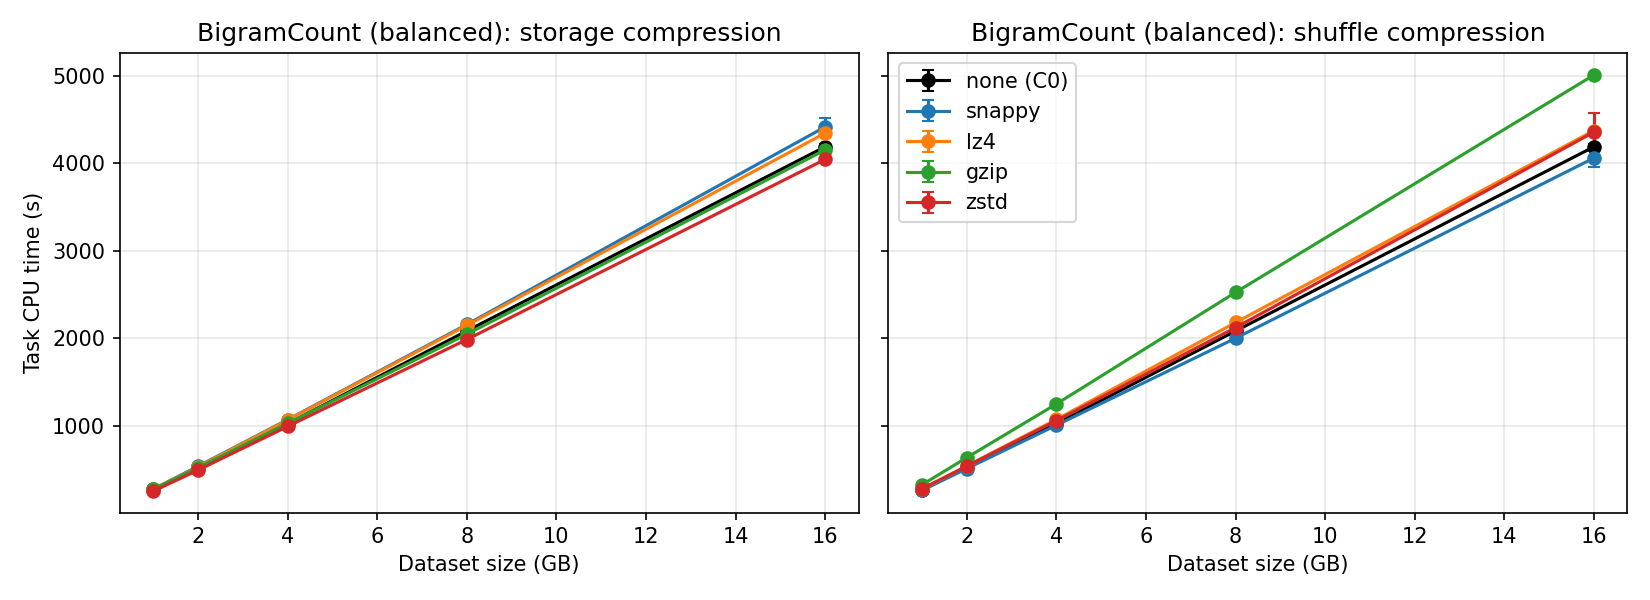
\includegraphics[width=0.9\linewidth]{../results/figures/cpu_vs_size_bigram.png}
  \caption{BigramCount: total task CPU time against dataset size.}

\end{figure}

\section{Discussion}
\subsection{Answers to the questions of the project}
\paragraph{1. Which codecs give the best trade-off between ratio and CPU overhead?}\mbox{}\\
Zstandard at level 3. In the micro-benchmark it has the best ratio of the four codecs (2.59) for 6.6 CPU seconds per GB, which is 2 to 2.5 times the cost of Snappy and LZ4 but 5 times less than Gzip. In the cluster it gave the shortest execution time in 5 of the 6 combinations of Sort or BigramCount with C1, C2 or C3 (the exception is BigramCount in C2, where Snappy was faster), and it added at most 24\% of CPU time (Sort, C2), against 124\% for Gzip. Snappy and LZ4 have the lowest CPU cost but a ratio of only about 1.55; they are a safe choice when CPU is scarce, and in our runs they behaved almost the same. Gzip is the worst trade-off: Zstandard compresses better and much faster, and Gzip doubles the CPU time of Sort when it is used for the shuffle.

\paragraph{2. Does compression systematically improve I/O-bound applications?}\mbox{}\\
Almost, but not systematically. For Sort, all 32 combinations of codec, size and C1 or C3 are faster than C0, by 12\% to 58\%. With C2 alone, the gain is small and not always present: Sort with Gzip in C2 was 7\% slower at 2 GB, LZ4 5\% slower at 2 GB, and Snappy only 2\% faster at 8 GB. The benefit depends on which bytes are compressed: compressing the HDFS input and output of Sort helps a lot, while compressing only the shuffle helps less because it adds CPU work in the maps and leaves the largest transfers unchanged.

\paragraph{3. How does compression affect CPU-bound applications?}\mbox{}\\
It does not help and it can slow them down. HashScore spends almost all of its CPU time computing hashes; it reads 8.4 GiB but shuffles almost nothing. Storage compression reduces the bytes read but this was not the bottleneck, so the execution time stays within the variation (between -1\% and +7\% at 8 GB). With Gzip or Zstandard in C3 it is 9 to 11\% slower, and at 1 GB up to 24\% slower. The extra CPU time is small (+4\% with Gzip) but every second of CPU taken by the codec is a second not used for hashing, because the CPUs are already saturated.

\paragraph{4. How do the benefits evolve with increasing dataset sizes?}\mbox{}\\
For the I/O-bound and balanced applications the relative gain is about constant between 1 and 8 GB, so the absolute time saved grows with the data (Table 5). For the CPU-bound application the overhead is largest at 1 GB and becomes small at 8 GB. Results at small sizes are also more variable (coefficients of variation up to 24\% at 1 to 2 GB). We could not check whether this stays true beyond 8 GB.

\paragraph{5. Is compression more beneficial for storage or for network communication?}\mbox{}\\
On our cluster it depends on where the bytes are. For Sort, storage compression is clearly more useful (-42\% with Zstandard in C1 against -14\% in C2 at 8 GB), because the input and the replicated output are larger than the shuffle and the output replicas also travel over the network. For BigramCount, whose output is small, the two levels give similar gains (-10\% to -16\% for C1 and -10\% to -23\% for C2). With a slower network, the value of shuffle compression goes up (Figure ??).

\paragraph{6. Can combining storage and communication compression degrade performance?}\mbox{}\\
Yes. C3 with Gzip is slower than C1 with Gzip for Sort (396 s against 370 s at 8 GB, also at 2 GB), and C3 is the slowest configuration of HashScore with Gzip and Zstandard. In both cases the extra compression of the shuffle adds CPU time that is not paid back. With fast codecs (Zstandard, Snappy, LZ4) on I/O-bound or balanced jobs, C3 was always the best configuration.

\paragraph{7. Under which conditions should compression be disabled?}\mbox{}\\
From our measurements: when the job is CPU-bound and moves little data (HashScore), when the CPUs are already saturated, for the shuffle when the codec is slow (Gzip) and the network is fast, and for small inputs where the fixed cost of the job dominates and the gain is lost in the variation. For Sort and BigramCount there was no configuration where turning off compression completely was the best choice.

\subsection{Unexpected results}
\begin{itemize}
  \item During the first smoke tests the uncompressed baseline was actually compressed. Our code called \path{SequenceFileOutputFormat.setOutputCompressionType(BLOCK)}, and this method also sets \path{mapreduce.output.fileoutputformat.compress} to true, so Hadoop compressed the C0 data with its default codec (zlib). We noticed it because the C0 dataset was smaller than the Snappy one. We removed the call, regenerated all datasets and ran the whole campaign again.
  \item Writing a dataset is faster with compression than without, even with Gzip, because HDFS writes every block twice.
  \item The 100 Mbit/s link of the laptop node is the bottleneck of the reduce phase of Sort (Figure~\ref{fig:mon}). This makes compression more profitable than it would be on a cluster with a uniform 1 Gbit/s network.
  \item In C1, Zstandard did not cost more CPU than Snappy and LZ4 in the cluster, even though it is 2 to 2.5 times more expensive in the micro-benchmark, because the tasks have fewer bytes to read, write and checksum.
  \item LZ4 has a lower ratio than Snappy but much faster decompression; in the jobs, these two codecs gave nearly identical results.
\end{itemize}

\subsection{Limitations}
\begin{itemize}
  \item The cluster is small (3 workers, 10 vcores) and heterogeneous. worker3 is slower than the other workers, especially for SHA-256, and it is connected at 100 Mbit/s while worker1 and worker2 share a virtual switch.
  \item Two of the workers run on the same PC, so they share its CPU, memory bandwidth and SSD.
  \item The data is synthetic text. Real data that is already compressed (images, video) would give a ratio close to 1 and only the CPU cost would remain.
  \item Snappy and LZ4 run in Java (snappy-java, lz4-java) in Hadoop 3.4, while zlib and Zstandard use native libraries. This may favour Zstandard a little.
  \item We used only one Zstandard level (3) in the cluster, three repetitions per point, and sizes up to 8 GB.
  \item Only Hadoop MapReduce was tested, not Spark.
\end{itemize}

\section{Conclusion}
Compression is useful in Hadoop when the job moves a lot of data and the CPUs are not saturated. On our cluster, compressing both the HDFS data and the shuffle with Zstandard made the I/O-bound Sort 58\% faster and the balanced BigramCount 37\% faster at 8 GB, with almost no increase in CPU time. For the CPU-bound HashScore, compression brought nothing and could cost up to 11\% at 8 GB. Gzip is not a good choice for intermediate data, and Zstandard at a low level is a better choice than Gzip everywhere. The decision to compress should therefore be based on the profile of the job and on the infrastructure, in particular the network: on our cluster the slow link of one node made compression of the transferred data much more valuable.

\appendix
\section{Screenshots of the Hadoop web interfaces}
These screenshots were taken at the end of the main campaign. More screenshots, taken during the campaign and during the network-limited runs, are in \path{report/evidence/screenshots/}.

\begin{figure}[H]
  \centering
  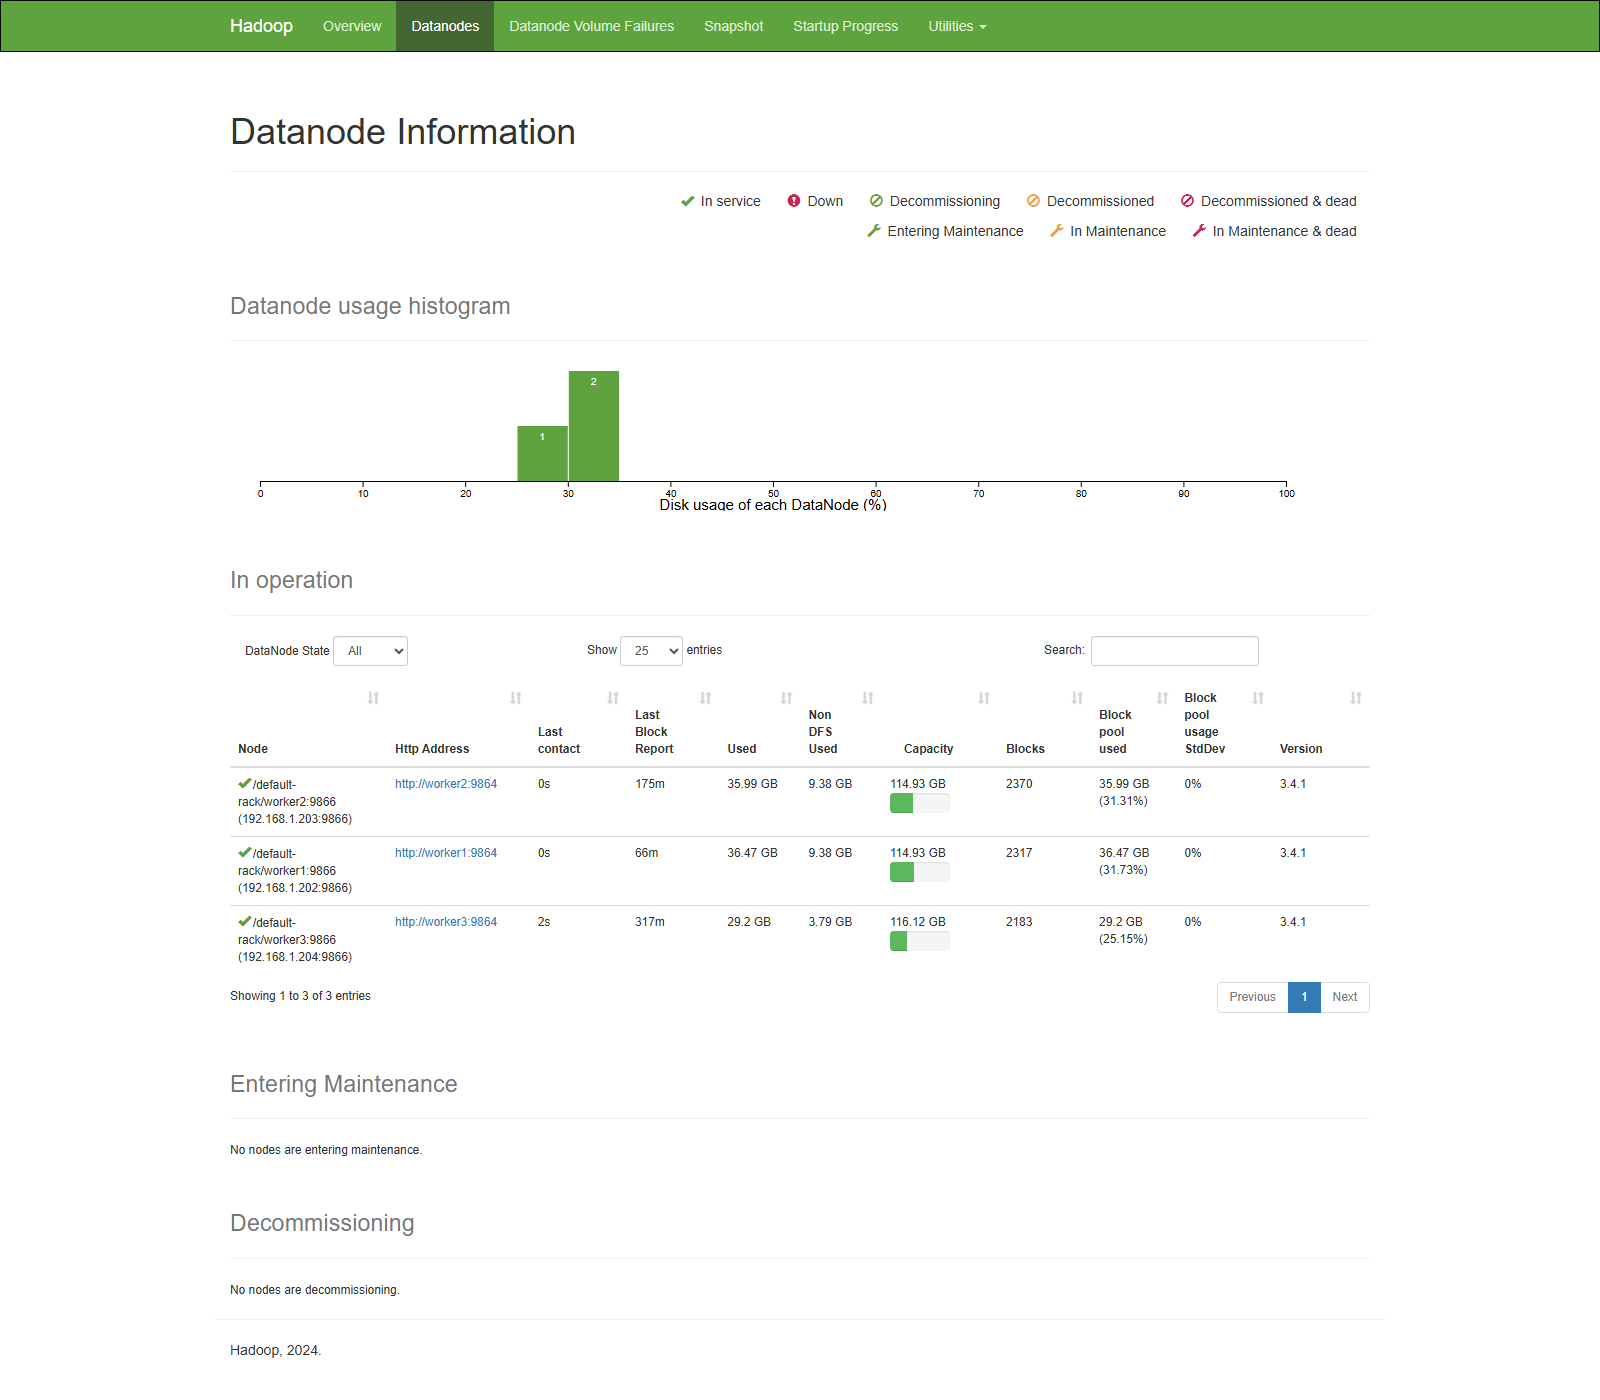
\includegraphics[width=0.8\linewidth]{evidence/screenshots/campaign-end/02_hdfs_datanodes.png}
  \caption{NameNode web UI: the three DataNodes and their disk usage.}

\end{figure}

\begin{figure}[H]
  \centering
  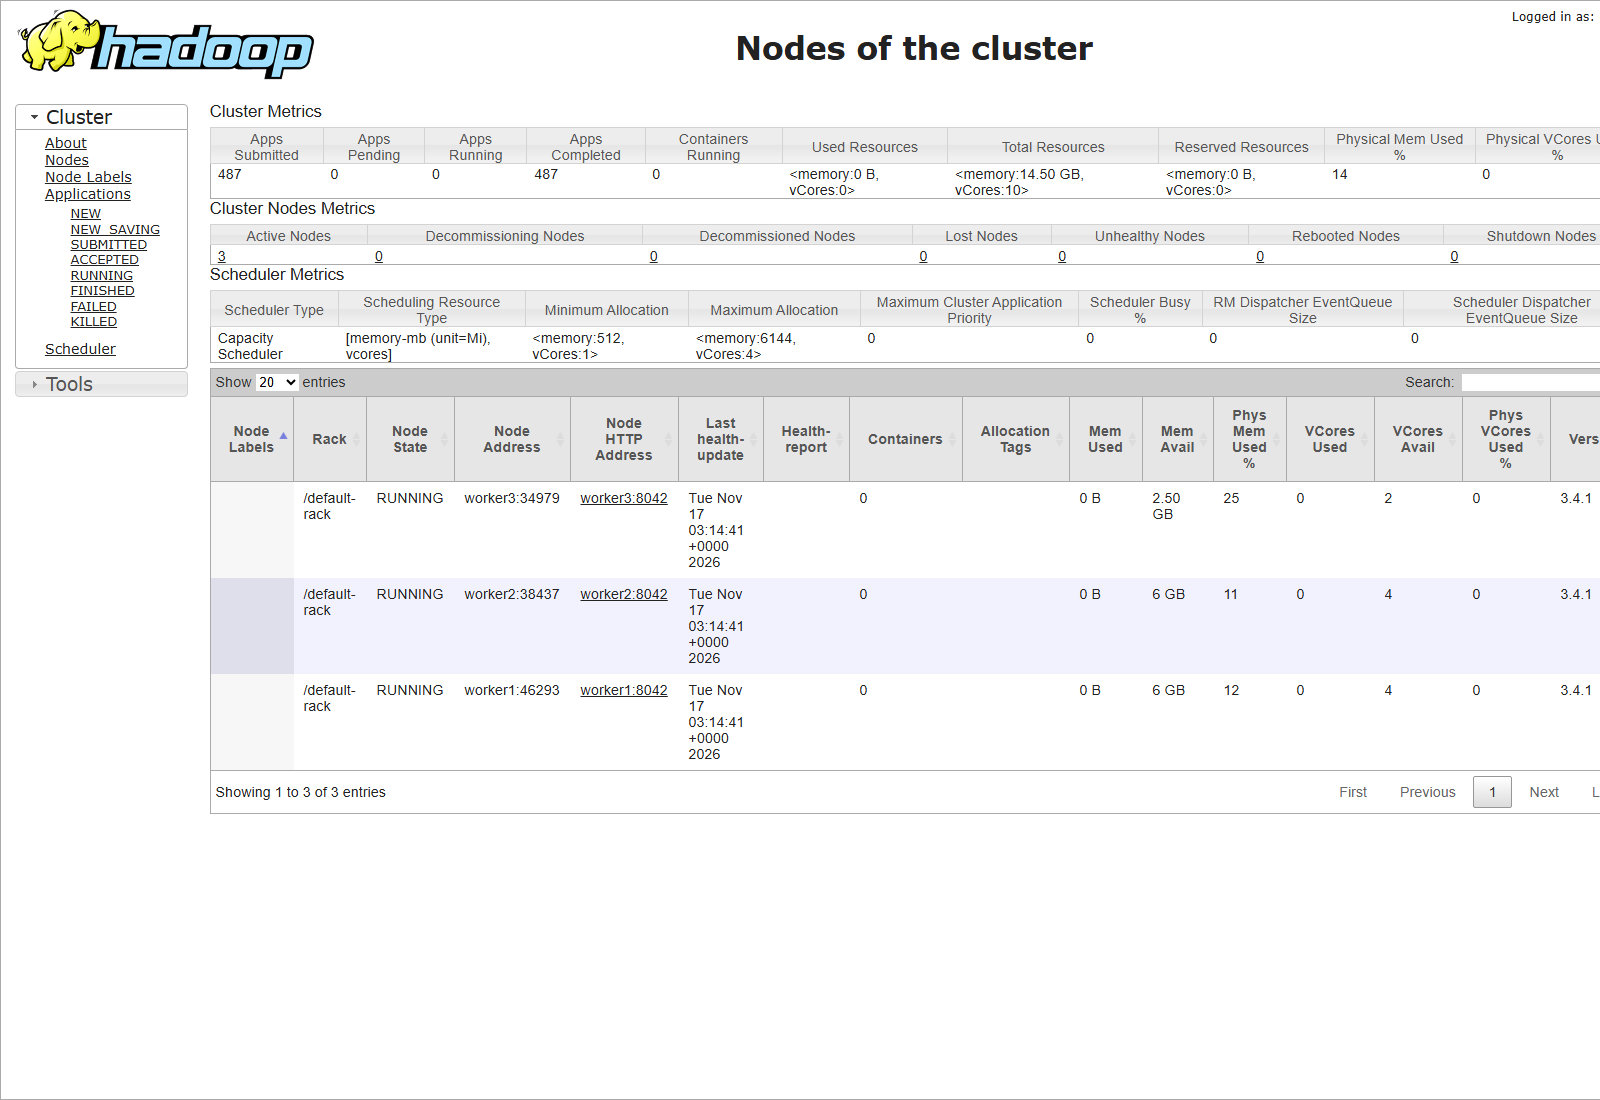
\includegraphics[width=0.8\linewidth]{evidence/screenshots/campaign-end/05_yarn_nodes.png}
  \caption{ResourceManager web UI: the three NodeManagers with their memory and vcores.}

\end{figure}

\begin{figure}[H]
  \centering
  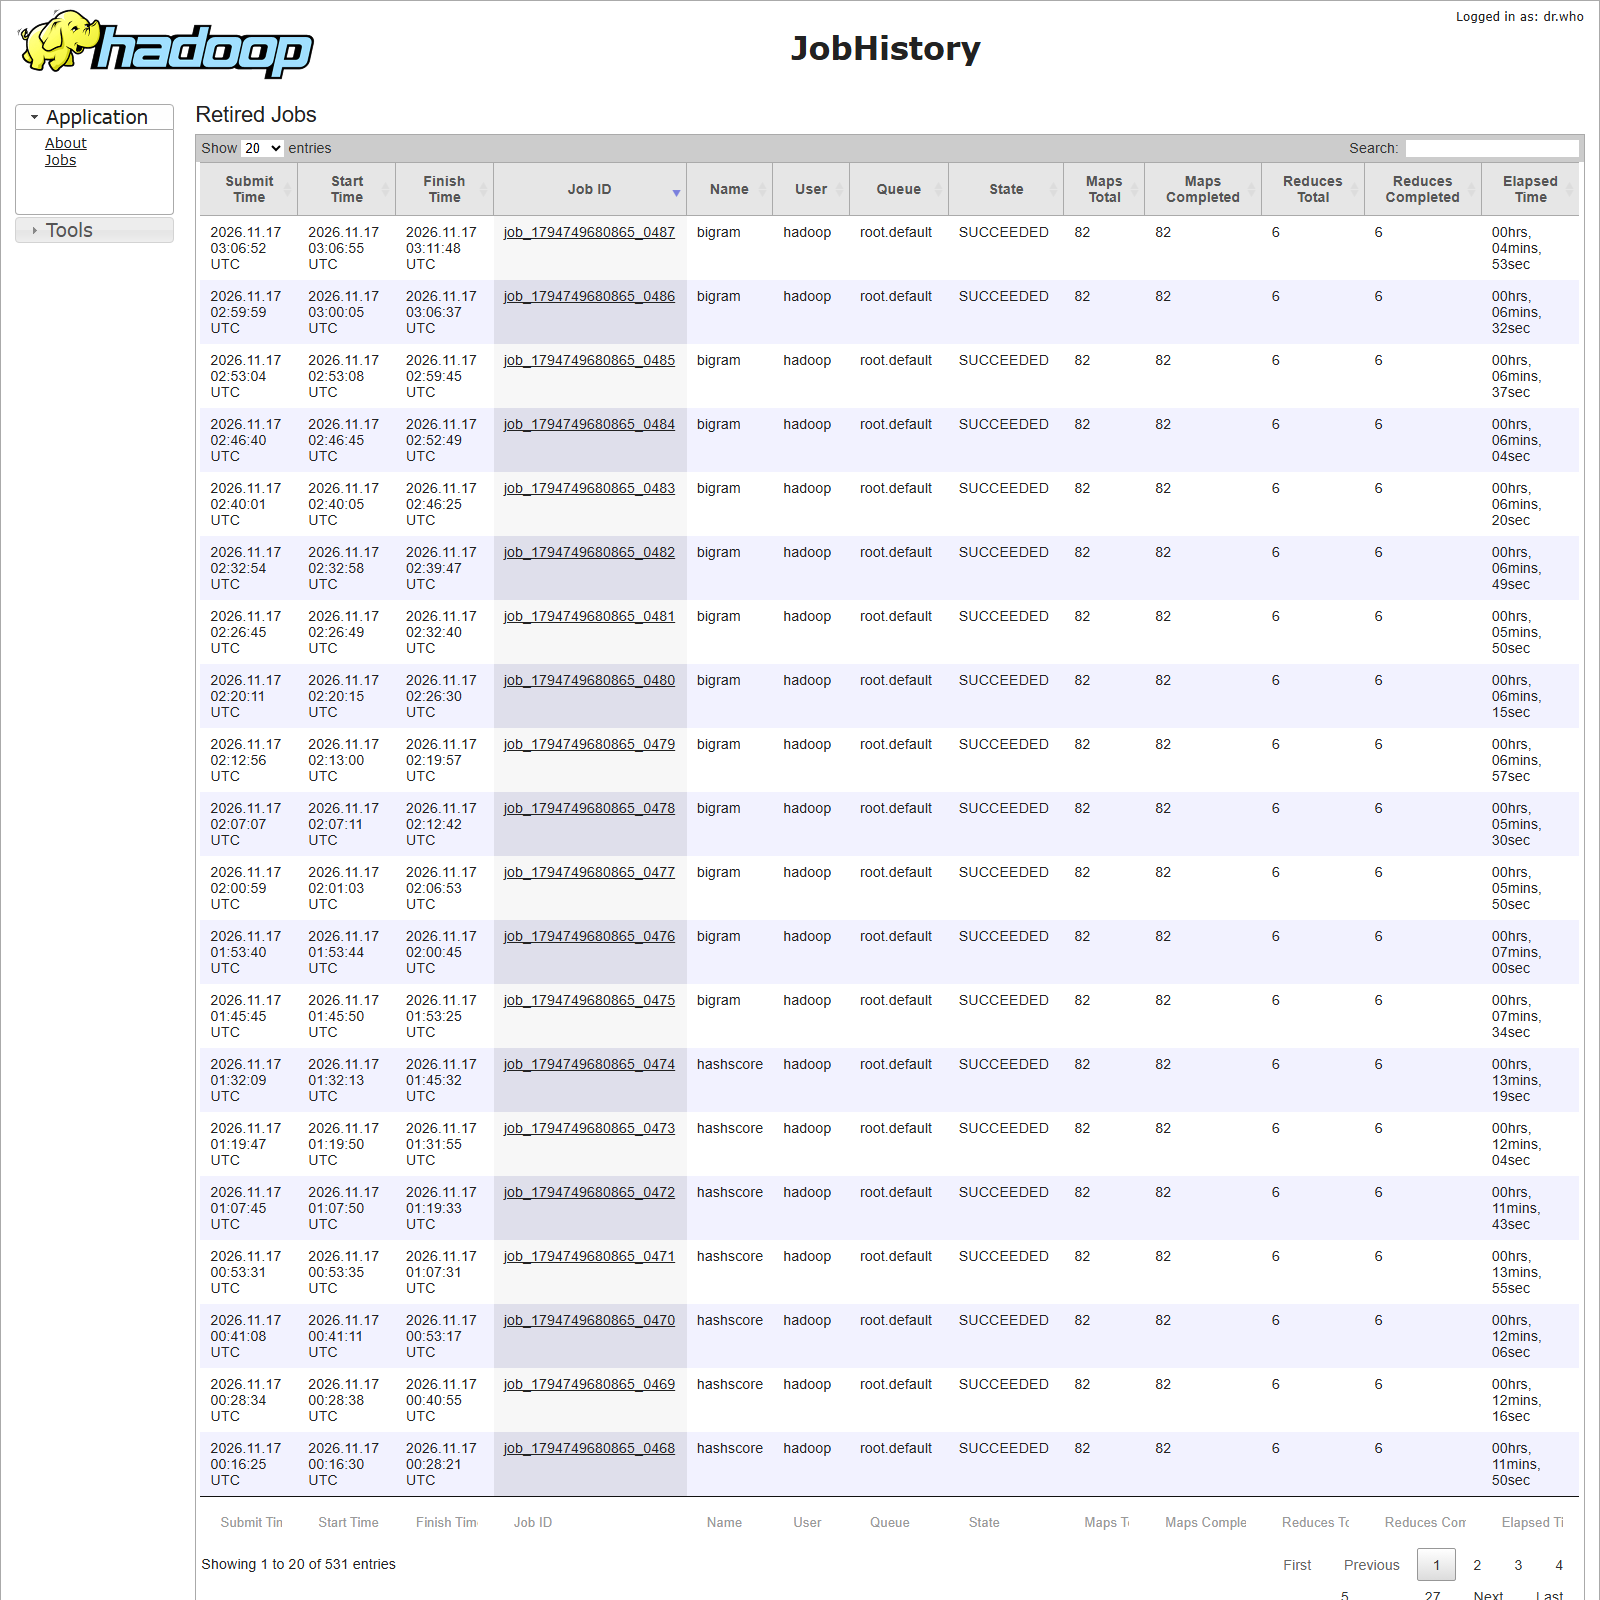
\includegraphics[width=0.8\linewidth]{evidence/screenshots/campaign-end/09_jobhistory.png}
  \caption{JobHistory server: list of finished jobs of the campaign.}

\end{figure}

\begin{figure}[H]
  \centering
  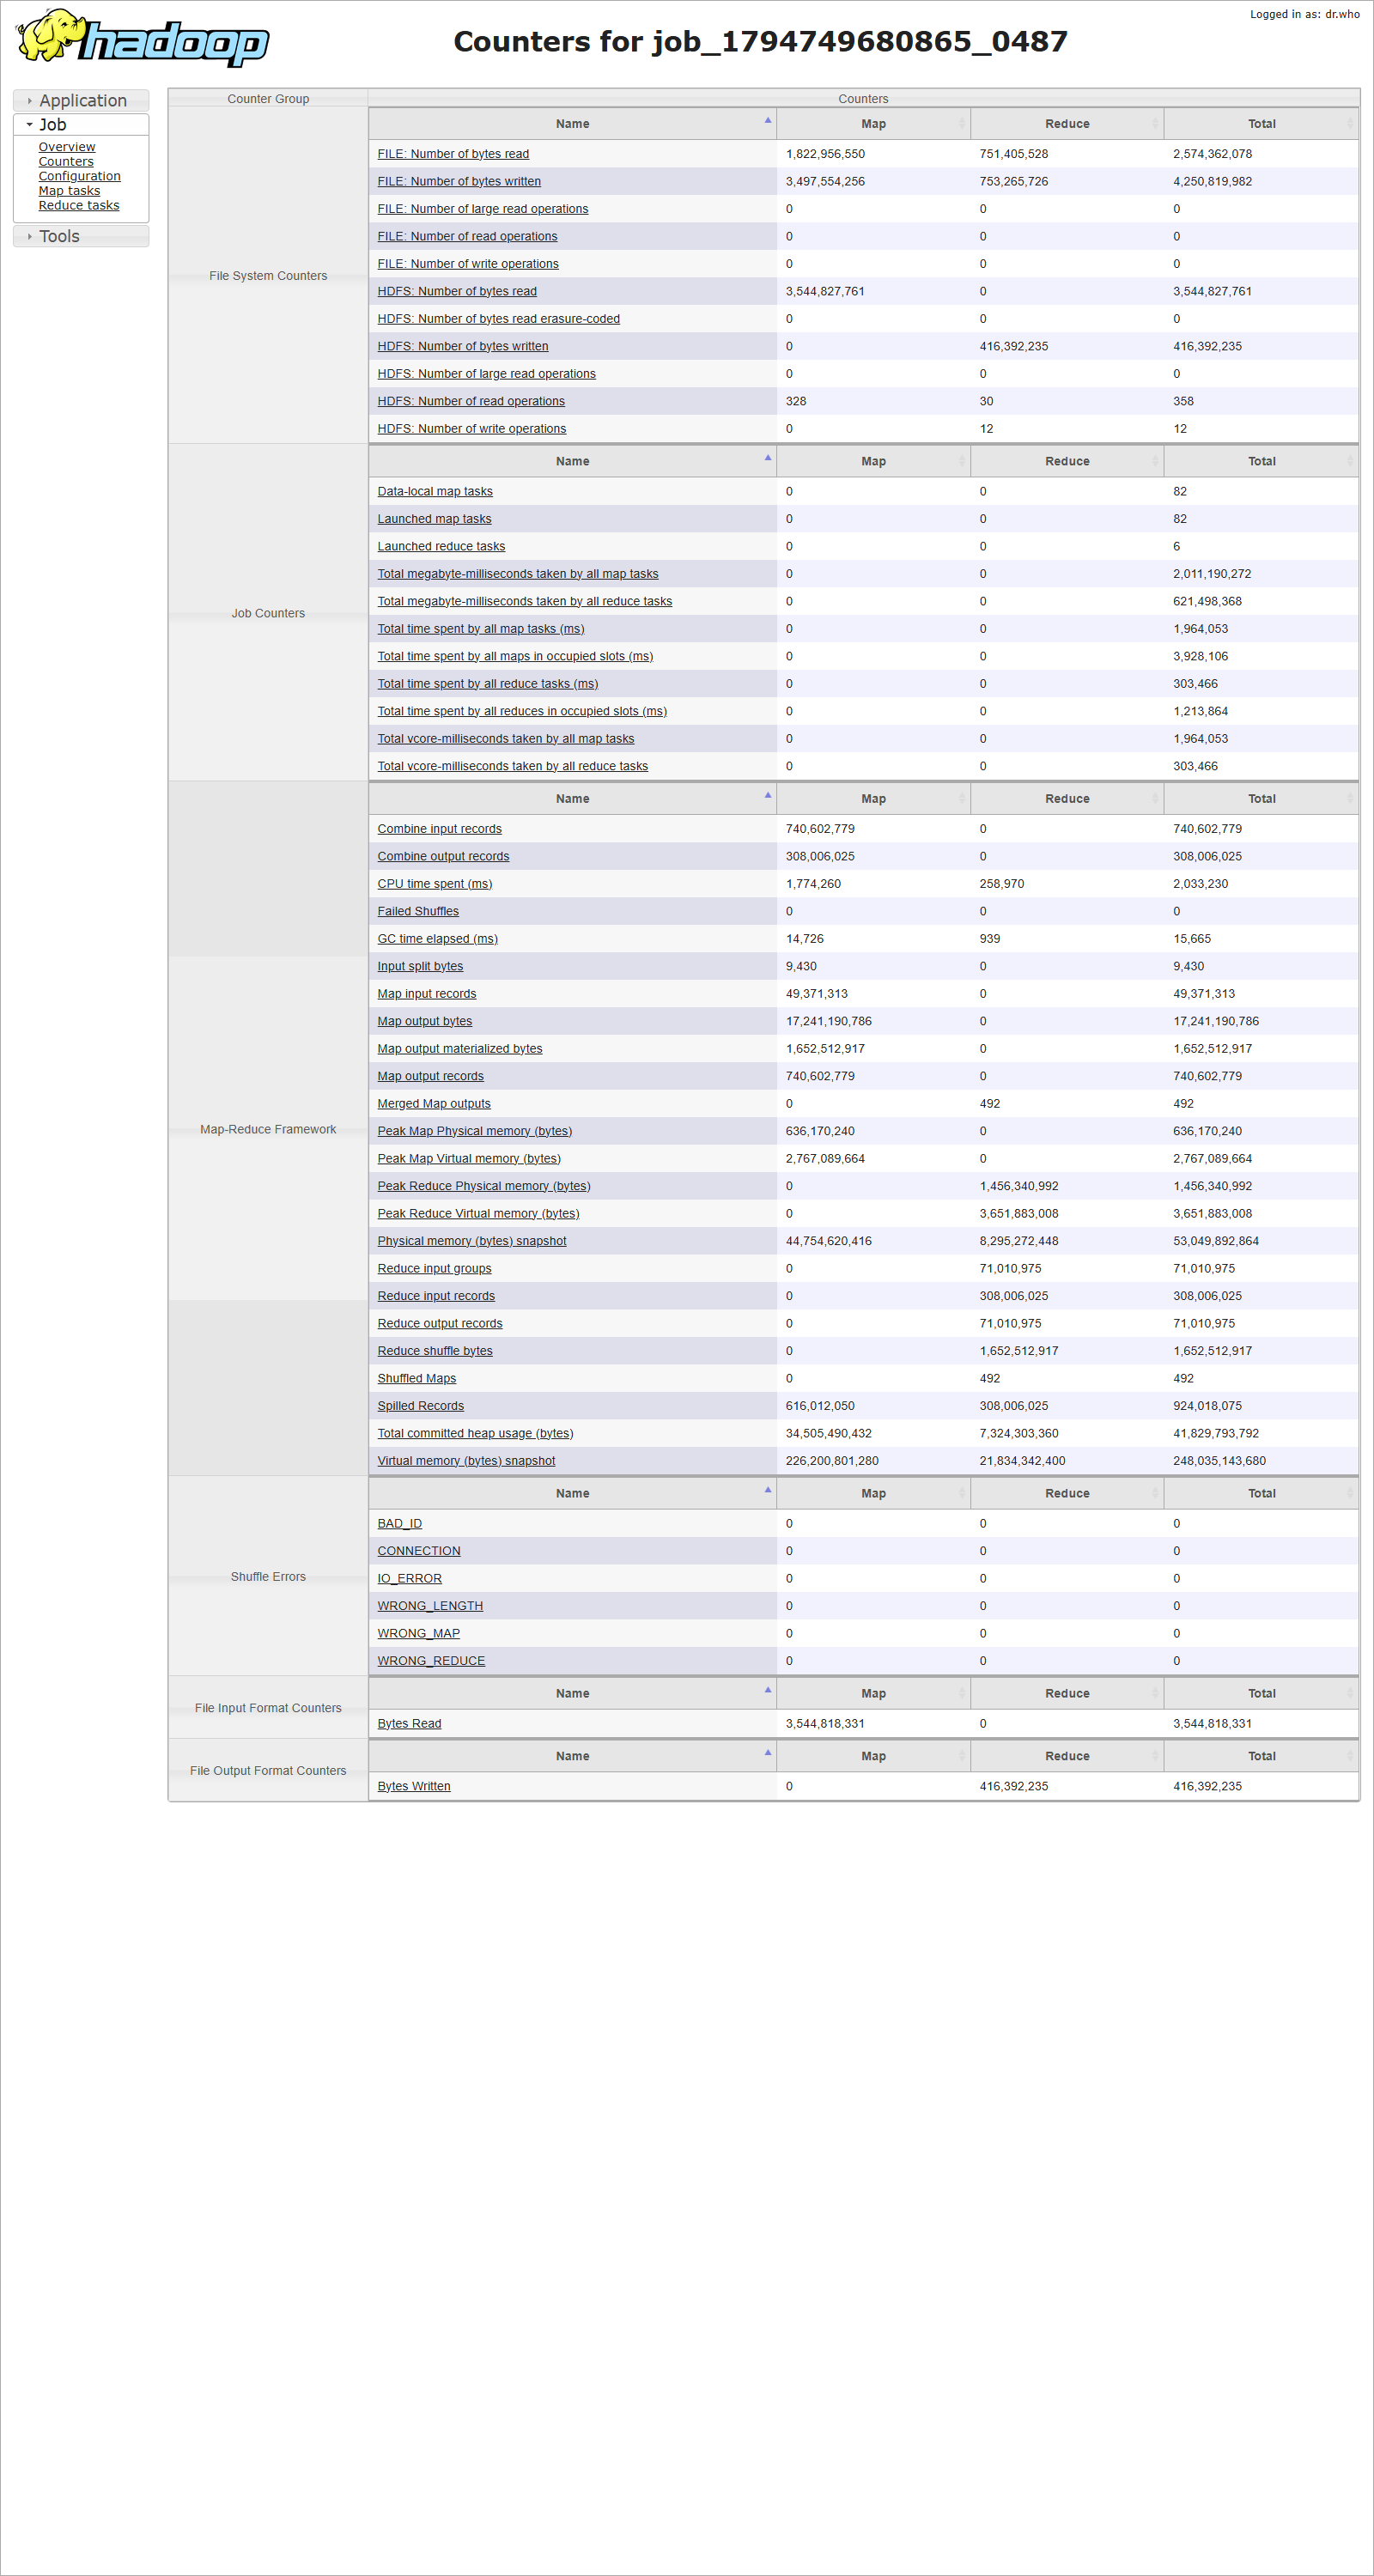
\includegraphics[width=0.6\linewidth]{evidence/screenshots/campaign-end/11_job_counters.png}
  \caption{Counters of one job in the JobHistory server, the source of the CPU time and shuffle bytes.}

\end{figure}

\section{How to reproduce}
\begin{verbatim}
cd ansible && ansible-playbook -i inventory.ini site.yml
cd ../apps && ./build.sh
cd .. && scripts/run_all.sh
scripts/netlimit.sh set 100mbit
RESULTS=$PWD/results-100mbit APPS="sort bigram" SIZES="2 4" CONFIGS=C2 scripts/run_experiments.sh
scripts/netlimit.sh clear
\end{verbatim}

\end{document}
